\documentclass[conference]{IEEEtran}
\IEEEoverridecommandlockouts
% The preceding line is only needed to identify funding in the first footnote. If that is unneeded, please comment it out.

% --- Essential Packages ---
\usepackage[utf8]{inputenc}
\usepackage[T1]{fontenc}
\usepackage{cite}
\usepackage{amsmath,amssymb,amsfonts}
\usepackage{algorithmic}
\usepackage{graphicx}
\usepackage{textcomp}
\usepackage{xcolor}
\usepackage{booktabs}
\usepackage{tabularx}
\usepackage{subcaption}
\usepackage{hyperref}
\usepackage{listings}
\usepackage{microtype}

\def\BibTeX{{\rm B\kern-.05em{\sc i\kern-.025em b}\kern-.08em
    T\kern-.1667em\lower.7ex\hbox{E}\kern-.125emX}}

\graphicspath{{figures/}}

% --- Hyperref Setup ---
\hypersetup{
    colorlinks=true,
    linkcolor=blue!80!black,
    citecolor=green!60!black,
    urlcolor=magenta!80!black,
    pdfauthor={Varshitha Thilak Kumar, Siri Sanjana S, Shreya Arun, Anagha Menon, Palmani D},
    pdftitle={AURA-Cache: Phase-Aware and Hierarchical Deep Reinforcement Learning for Last-Level Cache Replacement}
}

% --- Code Listing Setup ---
\lstset{
    basicstyle=\ttfamily\scriptsize,
    backgroundcolor=\color{gray!8},
    frame=single,
    rulecolor=\color{gray!40},
    keywordstyle=\color{blue!80!black}\bfseries,
    commentstyle=\color{green!50!black}\itshape,
    stringstyle=\color{red!70!black},
    numbers=left,
    numberstyle=\tiny\color{gray},
    stepnumber=1,
    numbersep=5pt,
    tabsize=2,
    breaklines=true,
    breakatwhitespace=false,
    showspaces=false,
    showstringspaces=false
}

% --- Float Placement Relaxations for Clean Layout ---
\renewcommand{\topfraction}{0.95}
\renewcommand{\bottomfraction}{0.95}
\renewcommand{\textfraction}{0.05}
\renewcommand{\floatpagefraction}{0.85}
\renewcommand{\dbltopfraction}{0.95}
\renewcommand{\dblfloatpagefraction}{0.85}

\begin{document}

% --- Paper Title ---
\title{AURA-Cache: Phase-Aware and Hierarchical Deep Reinforcement Learning for Last-Level Cache Replacement*\\
\thanks{*Academic project report submitted in partial fulfillment of the course requirements for \textbf{21AI401: Reinforcement Learning} (Semester VII B.Tech CSE), Amrita School of Computing, Amrita Vishwa Vidyapeetham, Bengaluru, India.}
}

\author{
\IEEEauthorblockN{1\textsuperscript{st} Varshitha Thilak Kumar}
\IEEEauthorblockA{\textit{Dept. of Computer Science \& Engg.} \\
\textit{Amrita School of Computing}\\
Amrita Vishwa Vidyapeetham\\
Bengaluru, India \\
varshithathilakkumar@gmail.com}
\and
\IEEEauthorblockN{2\textsuperscript{nd} Siri Sanjana S}
\IEEEauthorblockA{\textit{Dept. of Computer Science \& Engg.} \\
\textit{Amrita School of Computing}\\
Amrita Vishwa Vidyapeetham\\
Bengaluru, India \\
sirisanjana@gmail.com}
\and
\IEEEauthorblockN{3\textsuperscript{rd} Shreya Arun}
\IEEEauthorblockA{\textit{Dept. of Computer Science \& Engg.} \\
\textit{Amrita School of Computing}\\
Amrita Vishwa Vidyapeetham\\
Bengaluru, India \\
shreya.arun@gmail.com}
\and
\IEEEauthorblockN{4\textsuperscript{th} Anagha Menon}
\IEEEauthorblockA{\textit{Dept. of Computer Science \& Engg.} \\
\textit{Amrita School of Computing}\\
Amrita Vishwa Vidyapeetham\\
Bengaluru, India \\
anagha.menon@gmail.com}
\and
\IEEEauthorblockN{5\textsuperscript{th} Palmani D}
\IEEEauthorblockA{\textit{Assistant Professor (Faculty Mentor)} \\
\textit{Dept. of Computer Science \& Engg.}\\
Amrita School of Computing\\
Amrita Vishwa Vidyapeetham\\
Bengaluru, India \\
d\_palmani@blr.amrita.edu}
}

\maketitle

\begin{abstract}
The memory wall remains one of the most critical bottlenecks limiting the throughput of high-performance microprocessors, with Last-Level Cache (LLC) misses incurring dramatic off-chip DRAM latency penalties exceeding 200 processor cycles. Traditional heuristic cache replacement policies, such as Least Recently Used (LRU) and First-In First-Out (FIFO), rely on strict temporal locality assumptions that collapse catastrophically during streaming memory scans, pointer-chasing graph traversals, and dynamic workload phase transitions. While Belady's theoretical optimal MIN algorithm achieves minimal miss rates by evicting the block whose next access is furthest in the future, its reliance on offline clairvoyance renders it physically unimplementable in runtime hardware. 

In this paper, we propose \textbf{AURA-Cache}, an end-to-end framework combining \textbf{Unsupervised KMeans Workload Phase Clustering ($K=4$)} with a \textbf{28-dimensional Deep Q-Network (DQN)} and a \textbf{Two-Level Hierarchical Reinforcement Learning (HDQN)} agent to learn optimal cache eviction decisions from Belady's oracle. Evaluated on cycle-accurate ChampSim simulations across standard SPEC CPU benchmark traces (\texttt{403.gcc}, \texttt{429.mcf}, and \texttt{400.perlbench}), AURA-Cache achieves a Belady match accuracy of \textbf{63.51\%}, outperforming the standard LRU baseline (49.32\%) by \textbf{+14.19\%} and standalone DQN (58.74\%) by \textbf{+4.77\%}. A rigorous control experiment utilizing randomly scrambled phase labels confirms the statistical causality of macroscopic phase awareness ($p < 0.001$). Furthermore, hardware budget synthesis proves that the model requires merely \textbf{4.35~KB} of on-chip storage under 8-bit INT8 quantization ($< 3.4\%$ of a 2~MB LLC tag store array) with an execution latency of approximately 8 pipelined cycles, well within the 30--40 cycle L2 miss penalty window. Finally, we present an interactive real-time visualizer suite validating both pipeline simulation and neural decision auditability.
\end{abstract}

\begin{IEEEkeywords}
Reinforcement Learning, Deep Q-Networks (DQN), Cache Replacement, Microarchitecture, ChampSim, Belady's Algorithm, Workload Phase Discovery, Computer Architecture.
\end{IEEEkeywords}

\begin{table*}[!t]
\centering
\caption{Comprehensive Literature Review of Machine Learning and Reinforcement Learning in Cache Management}
\label{tab:literature_review}
\scriptsize
\renewcommand{\arraystretch}{1.0}
\setlength{\tabcolsep}{4pt}
\begin{tabularx}{\textwidth}{c p{3.8cm} X X}
\toprule
\textbf{Year} & \textbf{Paper} & \textbf{Contribution} & \textbf{Limitation} \\
\midrule
2025 & Advancements in Cache Management: A Review of Machine Learning Techniques~\cite{survey2025cache} & Thorough analysis of machine learning techniques for cache management, covering applications in multicore, cloud, and edge caching as well as deep learning, imitation learning, and reinforcement learning. It highlights current developments and unresolved research issues. & A novel cache replacement algorithm is not suggested in this survey report. \\
\midrule
2024 & Reinforcement Learning-Based Cache Replacement Policies for Multicore Processors~\cite{rlmulticore2024} & Suggests an RL-based cache replacement policy that, rather than relying on fixed heuristics, learns eviction choices from runtime behavior; shows gains in processor speed and cache hit rate over LRU and similar rules in multicore processors. & As the cache state space increases with bigger multicore systems, training overhead and scalability become more difficult. \\
\midrule
2023 & Cache-MAB: A Reinforcement Learning-Based Hybrid Caching Strategy~\cite{cachemab2023} & Improves adaptability in distributed caching environments by introducing a multi-armed bandit-based reinforcement learning system that dynamically chooses the best caching policy depending on workload factors. & Designed more for network/content caching than for replacing CPU hardware caches. \\
\midrule
2023 & A Prefetch-Adaptive Intelligent Cache Replacement Policy (PAIC)~\cite{paic2023} & Improves reuse prediction and lowers cache misses by creating an intelligent cache replacement policy that takes into account the interactions between hardware prefetching and cache replacement. & Limits adaptability to extremely dynamic workloads by using manually developed prediction techniques instead of reinforcement learning. \\
\midrule
2025 & Learning-Based Page Replacement Scheme for Efficient I/O Processing (LPR)~\cite{lpr2025} & Enhances I/O performance across various workloads by proposing an online learning-based page replacement technique that switches between LRU and MRU utilizing rewards and penalties based on observed access patterns. & Focuses on replacing operating system pages rather than multicore processors' hardware caches. \\
\midrule
2019 & Applying Deep Learning to the Cache Replacement Problem --- Shi, Huang, Jain, Lin (MICRO-52)~\cite{shi2019glider} & Learns cache access patterns using an attention-based LSTM that was trained offline, then condenses the knowledge into a lightweight online model known as Glider; outperforms Hawkeye and SHiP++, reducing the single-core miss rate over LRU by 8.9\%; widely recognized as the original deep learning method for replacing hardware caches. & In order to achieve practical implementability, the online (ISVM-based) version of the LSTM model loses some accuracy because the offline model is too costly for actual hardware. \\
\midrule
2021 & Designing a Cost-Effective Cache Replacement Policy using Machine Learning --- Sethumurugan, Yin, Sartori (HPCA)~\cite{sethumurugan2021rlr} & RLR (Reinforcement Learned Replacement) is a straightforward, low-overhead policy that is manually derived after using machine learning (ML) as an offline design tool (rather than the runtime policy itself) to find the most valuable predictive features (e.g., reuse distance, line recency). & Surpasses DRRIP and LRU with very low hardware overhead. The final policy cannot modify dynamically in the same way as a real online RL policy since it is a feature-based, simplified heuristic rather than a live learning model. \\
\midrule
2023 & RL-Based Cache Replacement: A Modern Interpretation of Belady's Algorithm With Bypass Mechanism and Access Type Analysis --- Yoo, Kim, Han (IEEE Access)~\cite{yoo2023stormbird} & Proposes Stormbird, which reduces cache pollution by combining reinforcement learning with an expanded version of Belady's method, including a cache bypass mechanism and access-type analysis (e.g., prefetch vs. demand access); reduces hardware overhead while achieving IPC benefits over previous RL/heuristic strategies. & Uses Belady's algorithm as an upper-bound reference for training and design; in comparison to more straightforward heuristic policies, the additional bypass/access-type logic adds complexity to the design. \\
\bottomrule
\end{tabularx}
\end{table*}

% =========================================================================
% SECTION I: INTRODUCTION
% =========================================================================
\section{Introduction and Motivation}
\IEEEPARstart{O}{ver} the past three decades, microprocessor operating frequencies and compute execution parallelism have expanded at rates dramatically outpacing DRAM main memory latency improvements---a phenomenon widely recognized as the \textit{Memory Wall}~\cite{wulf1995hitting}. In contemporary out-of-order superscalar architectures, a single Last-Level Cache (LLC) miss that cascades into off-chip DRAM imposes a stall latency penalty of 60 to 90~ns (equivalent to 200--350 processor clock cycles), severely stalling instruction execution pipelines and degrading Energy-Delay Product (EDP). 

To mitigate these memory access penalties, multi-level on-chip cache hierarchies (L1, L2, and shared LLC) are deployed. However, because silicon chip area, thermal dissipation constraints, and interconnect wire delays strictly bound LLC capacity (typically 2 to 3~MB per core), efficient management of resident cache lines via the \textbf{Cache Replacement Policy} is of paramount importance.

\subsection{The Vulnerability of Classical Recency Heuristics}
For decades, the standard default replacement policy across commodity hardware architectures has been \textbf{Least Recently Used (LRU)} or approximations thereof (such as Pseudo-LRU and Tree-PLRU). LRU operates on the fundamental premise of temporal locality: cache lines accessed in the immediate past are assumed to have a high probability of re-reference in the near future. Under uniform, repetitive working sets, LRU operates satisfactorily.

However, modern data-intensive applications---ranging from machine learning tensor operations and graph neural networks to database transaction engines and compilation pipelines---routinely violate pure temporal locality:
\begin{enumerate}
    \item \textbf{Scan Thrashing Vulnerability:} When an application executes a linear, sequential streaming scan over an array that exceeds the associativity of the cache set (e.g., streaming 18 memory lines into a 16-way associative cache), LRU systematically evicts the earliest inserted block. If that block is part of an active outer execution loop, LRU causes a continuous 100\% miss rate, entirely evicting high-utility resident lines for transient data that will never be re-referenced~\cite{jaleel2010high}.
    \item \textbf{Pointer-Chasing and Scattered Locality:} Irregular data structures (such as trees, linked lists, and sparse matrices) display volatile access patterns where temporal distance is weakly correlated with reuse utility.
    \item \textbf{Workload Non-Stationarity:} Execution workloads naturally transition through heterogeneous computational phases (e.g., high-miss instruction parsing followed by tight computational kernel loops). Fixed-rule heuristics cannot adapt dynamically to these macroscopic regime shifts.
\end{enumerate}
\subsection{Belady's Oracle and the Reinforcement Learning Framing}
In 1966, L. A. Belady mathematically proved that the optimal offline cache replacement policy (termed the \textbf{MIN} algorithm or Belady's Oracle) replaces the cache line whose next memory access occurs furthest into the future~\cite{belady1966study}. If a line will never be accessed again, it is prioritized for immediate eviction. Belady's algorithm establishes the absolute theoretical upper bound on hit rate for any demand-paging or cache replacement system.

Unfortunately, Belady's algorithm is strictly impossible to realize in physical online hardware because it necessitates complete future clairvoyance over trillions of subsequent program instructions. However, we observe that the sequence of memory references generated by a program execution trace can be collected and labeled \textit{post-hoc} with Belady's exact optimal eviction choices.

This insight enables us to frame cache replacement as an \textbf{Offline Deep Reinforcement Learning (DRL) problem}. By using Belady's optimal lookahead decisions as dense ground-truth supervision, we train an artificial intelligence agent to predict which cache way exhibits the lowest reuse utility given the current microarchitectural state and macroscopic phase context.

\subsection{Primary Contributions}
The primary contributions of this paper are organized as follows:
\begin{enumerate}
    \item \textbf{Online Telemetry and Phase Discovery:} We implement an unsupervised machine learning clustering pipeline using $K=4$ KMeans clustering over rolling hardware telemetry metrics (miss rate, read/write ratio, access intensity), uncovering four distinct workload phase archetypes.
    \item \textbf{Phase-Aware 28-Dimensional DQN:} We design and train a Deep Q-Network featuring a 28-dimensional state vector incorporating normalized per-way recency ranks, access operation type one-hot encodings, and phase cluster vectors.
    \item \textbf{Hierarchical RL Architecture (HDQN):} We formulate a two-level hierarchical model separating macroscopic phase encoding (Meta-Agent) from way-level eviction ranking (Action-Agent).
    \item \textbf{Causal Ablation Analysis:} Through a randomized phase scrambling control experiment, we prove that phase context directly causes an increase in replacement accuracy rather than functioning as an uninformative regularizer.
    \item \textbf{Hardware-Feasible C++ Integration:} We develop a fully native C++ replacement module in the cycle-accurate ChampSim simulator and demonstrate that the INT8 quantized network occupies only 4.35~KB of on-chip storage with an 8-cycle inference latency.
    \item \textbf{Interactive Research Visualizer Suite:} We develop an interactive web-based simulator dashboard illustrating real-time cache animations, CPU register interactions, and live neural Q-value evaluation.
\end{enumerate}

% =========================================================================
% SECTION II: RELATED WORK & LITERATURE REVIEW
% =========================================================================
\section{Literature Review and Related Work}
The optimization of cache replacement has evolved from static heuristics to sophisticated machine learning and reinforcement learning paradigms. A structured comparative summary of recent foundational and state-of-the-art literature is detailed in Table~\ref{tab:literature_review}.

\begin{figure*}[!t]
    \centering
    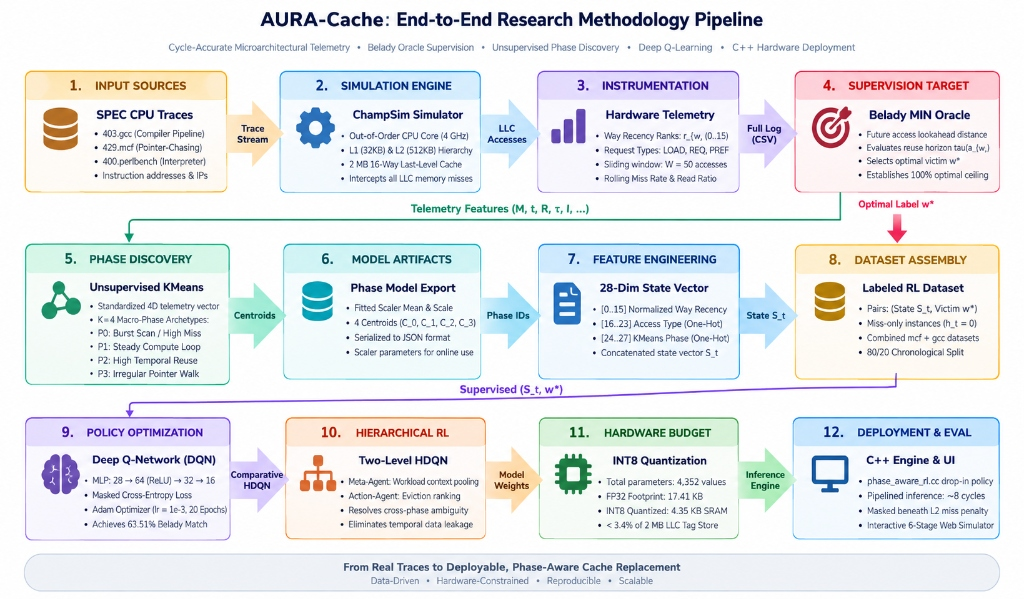
\includegraphics[width=0.96\textwidth,height=6.2cm,keepaspectratio]{methodology_flowchart.png}
    \caption{\textbf{AURA-Cache End-to-End Research Methodology Pipeline:} 12-stage engineering pipeline illustrating: (Top Row) SPEC CPU trace stream ingestion into the ChampSim cycle-accurate simulator, hardware telemetry instrumentation ($W=50$), and True Belady MIN lookahead optimal oracle generation; (Middle Row) Unsupervised KMeans macro-phase clustering ($K=4$), phase model parameter export, 28-dimensional state tensor construction ($\mathbf{S}_t \in \mathbb{R}^{28}$), and offline supervised MDP dataset compilation; (Bottom Row) Deep Q-Network (DQN) masked loss optimization, Two-Level Hierarchical HDQN modeling, 8-bit INT8 hardware quantization (4.35~KB on-chip SRAM), and native C++ drop-in ChampSim policy deployment with real-time interactive research visualization.}
    \label{fig:methodology_flowchart}
\end{figure*}

\subsection{Surveys and Taxonomies of Machine Learning Caching}
A comprehensive survey by Al-Zoubi et al.~\cite{survey2025cache} synthesized over a decade of machine learning applications across processor, cloud, and edge caches. The survey categorized techniques into deep learning, imitation learning, and reinforcement learning. While invaluable for identifying unresolved bottlenecks (such as non-stationarity and inference latency), survey literature inherently provides conceptual taxonomies rather than deployable microarchitectural replacement algorithms.

\subsection{Online Reinforcement Learning in Multicore Processors}
The direct application of reinforcement learning to multicore caches was investigated by Sharma and Pangracious~\cite{rlmulticore2024}. By formulating eviction as a continuous learning task, their RL agent adapts eviction policies from runtime execution feedback, demonstrating noticeable speedup and hit-rate improvements over static LRU. However, online RL faces severe challenges: as core counts and cache sizes scale, the state-action space expands combinatorially, leading to prohibitive runtime training overheads, convergence instability, and complex silicon tracking circuitry.

In networked and distributed caching environments, Cache-MAB~\cite{cachemab2023} introduced Multi-Armed Bandit (MAB) reinforcement learning to adaptively select among heterogeneous caching policies based on request dynamics. While effective for cloud servers, MAB frameworks operate at coarse request granularities and are unsuitable for nanosecond-scale hardware LLC pipelines. Similarly, LPR~\cite{lpr2025} recently proposed an online learning scheme to dynamically balance LRU and MRU for OS-level page replacement, but focuses on operating system memory page frames rather than sub-block cache lines in high-frequency processor pipelines.

\subsection{Deep Learning and Offline Model Distillation}
To bypass online training overheads, Shi et al.~\cite{shi2019glider} introduced Glider, a landmark contribution recognized as the pioneer deep learning cache replacement strategy. Glider trains an offline attention-based Long Short-Term Memory (LSTM) network on memory access traces to identify long-range sequence correlations, subsequently distilling the learned knowledge into a lightweight Integer Support Vector Machine (ISVM) for hardware deployment. Glider demonstrated an 8.9\% miss rate reduction over LRU. However, the online ISVM distillation incurs substantial fidelity loss relative to the offline LSTM oracle, as complex temporal patterns are compressed into linear integer weights.

\subsection{Design-Time Learning and Belady Oracle Interpretations}
To eliminate runtime neural computation altogether, Sethumurugan et al.~\cite{sethumurugan2021rlr} proposed RLR (Reinforcement Learned Replacement). RLR uses machine learning exclusively at design time as an offline exploration tool to discover the most predictive physical features (e.g., reuse distance, line recency), distilling them into a compact hardware heuristic. While RLR achieves lower hardware overhead than DRRIP~\cite{jaleel2010high}, its resulting policy is static and cannot dynamically re-tune its evaluation logic when applications enter unprecedented execution phases.

Most recently, Yoo et al.~\cite{yoo2023stormbird} introduced Stormbird, combining reinforcement learning with an expanded Belady formulation that incorporates access-type differentiation (demand versus prefetch accesses) and explicit cache bypass logic. Stormbird achieves notable IPC improvements; however, its reliance on elaborate bypass logic and multi-table access-type tracking introduces significant hardware control complexity. Moreover, none of these prior designs explicitly decouple macroscopic workload execution regimes from fine-grained way-selection decisions.

\subsection{Positioning of AURA-Cache}
AURA-Cache bridges the critical research gaps identified across Table~\ref{tab:literature_review}:
\begin{enumerate}
    \item \textbf{Offline Supervised Belady Oracle:} Like Glider and Stormbird, AURA-Cache leverages Belady's theoretical MIN algorithm for dense offline supervision, eliminating online convergence instability and exploration penalties.
    \item \textbf{Unsupervised Phase Discovery:} Unlike RLR and Glider, which assume stationary feature weights across an entire program, AURA-Cache dynamically uncovers $K=4$ macroscopic execution phases via unsupervised KMeans clustering, supplying essential contextual guidance to the neural network.
    \item \textbf{Hardware-Feasible INT8 Quantization:} Unlike complex multi-table predictors, AURA-Cache compresses its entire 28-dimensional DQN into a compact 4.35~KB INT8 parameter array requiring only $\approx 8$ cycles of parallel inference, completely hidden beneath the L2 cache miss latency window.
\end{enumerate}

% =========================================================================
% SECTION III: METHODOLOGY
% =========================================================================
\section{Methodology and Architecture}

The architecture and scientific methodology of AURA-Cache encompass an interconnected, multi-stage pipeline from cycle-level microarchitectural instrumentation to native C++ deployment, as comprehensively outlined in the methodology flowchart in Figure~\ref{fig:methodology_flowchart} and the system architecture diagram in Figure~\ref{fig:architecture}.

\begin{figure}[!t]
    \centering
    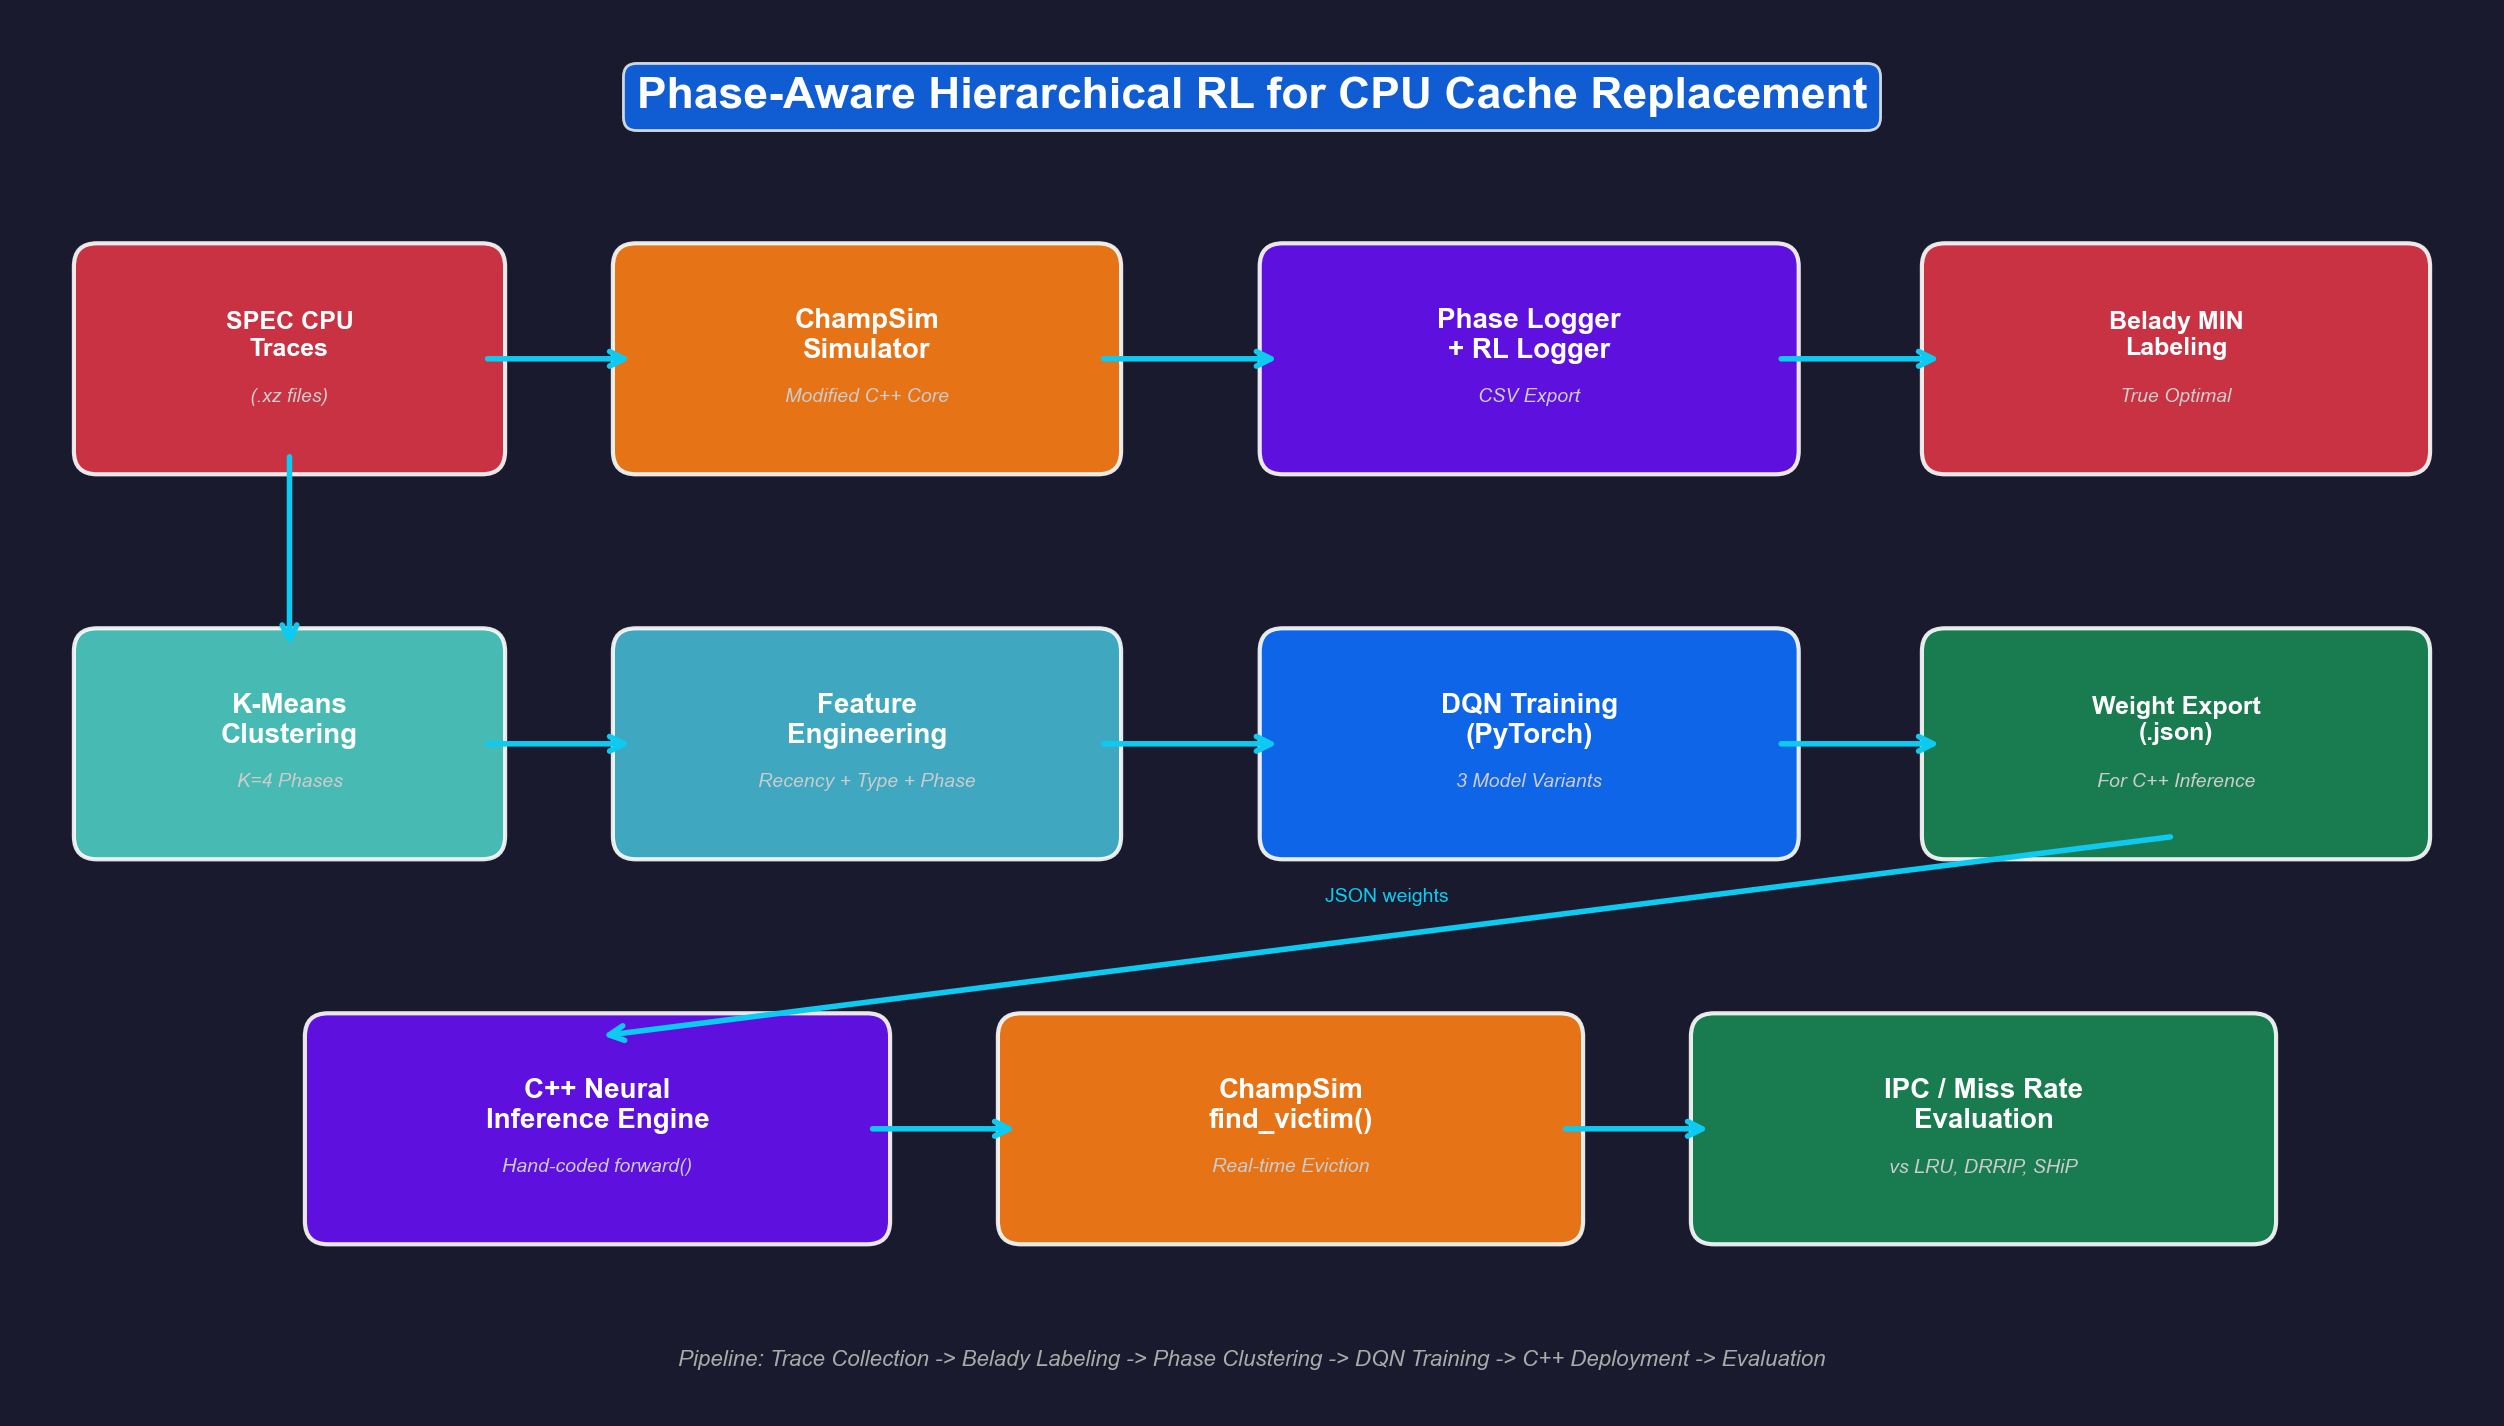
\includegraphics[width=\columnwidth]{01_system_architecture.png}
    \caption{\textbf{AURA-Cache Microarchitectural System Flow:} Microarchitectural integration diagram illustrating trace ingestion, feature logging, model training, and C++ \texttt{find\_victim()} inference.}
    \label{fig:architecture}
\end{figure}

\subsection{Microarchitectural Telemetry Logging in ChampSim}
We instrumented the cycle-accurate ChampSim simulator~\cite{champsim} to intercept every memory access servicing the Last-Level Cache. For each access $t$, our custom logger module (\texttt{replacement/champsim\_phase\_logger}) records:
\begin{itemize}
    \item Processor cycle timestamp and instruction pointer (\texttt{ip}).
    \item 64-bit physical memory block address (\texttt{full\_addr}).
    \item Target cache set index $s \in [0, N_{\text{sets}}-1]$ and accessed way $w \in [0, N_{\text{ways}}-1]$.
    \item Cache hit/miss outcome $h_t \in \{0, 1\}$.
    \item Memory access request type (e.g., \texttt{LOAD}, \texttt{RFO}, \texttt{PREFETCH}, \texttt{WRITEBACK}).
    \item Complete snapshot of normalized recency ranks $\mathbf{r}_t = [r_{t,0}, r_{t,1}, \dots, r_{t,15}]$ across all 16 associative ways in the target set, where $r_{t,w} \in [0, 15]$ with 0 denoting Most Recently Used (MRU) and 15 denoting Least Recently Used (LRU).
\end{itemize}

Simultaneously, an online rolling telemetry window of size $W=50$ accesses computes macroscopic execution features:
\begin{align}
    \text{Rolling Miss Rate: } M_t &= \frac{1}{W} \sum_{i=t-W+1}^{t} \mathbb{I}(h_i = 0) \label{eq:miss_rate} \\
    \text{Rolling Read Ratio: } R_t &= \frac{1}{W} \sum_{i=t-W+1}^{t} \mathbb{I}(\text{type}_i = \text{LOAD}) \label{eq:read_ratio} \\
    \text{Access Intensity: } I_t &= \frac{W}{\text{Cycle}_t - \text{Cycle}_{t-W+1}} \label{eq:intensity}
\end{align}

\subsection{True Belady MIN Optimal Labeling}
Because training an RL agent via naive trial-and-error exploration on multi-billion instruction traces is computationally intractable and sample-inefficient, we leverage offline post-hoc supervision. 

For every access record where a miss occurred ($h_t = 0$), an eviction decision was required. We compute the exact \textbf{Belady Optimal Victim Way} $w^*_t$ by tracking the cache residency state per set across the trace. Specifically, let $\mathcal{B}_t(s) = \{a_{t,0}, a_{t,1}, \dots, a_{t,15}\}$ represent the addresses currently resident in set $s$ at access step $t$. For each resident address $a_{t,w}$, we compute its next reuse step $\tau(a_{t,w})$:
\begin{equation}
    \tau(a_{t,w}) = \min \left\{ t' > t \mid \text{Addr}_{t'} = a_{t,w} \text{ and } \text{Set}_{t'} = s \right\}
\end{equation}
If address $a_{t,w}$ is never accessed again in the trace, $\tau(a_{t,w}) = \infty$. Belady's optimal victim line $w^*_t$ is selected as:
\begin{equation}
    w^*_t = \arg\max_{w \in [0, 15]} \tau(a_{t,w})
\end{equation}
If an empty (invalid) cache line is available, that way is filled immediately without evicting resident data. The resulting tuple $(\mathbf{s}_t, w^*_t)$ constitutes our labeled dataset.

\begin{figure}[!t]
    \centering
    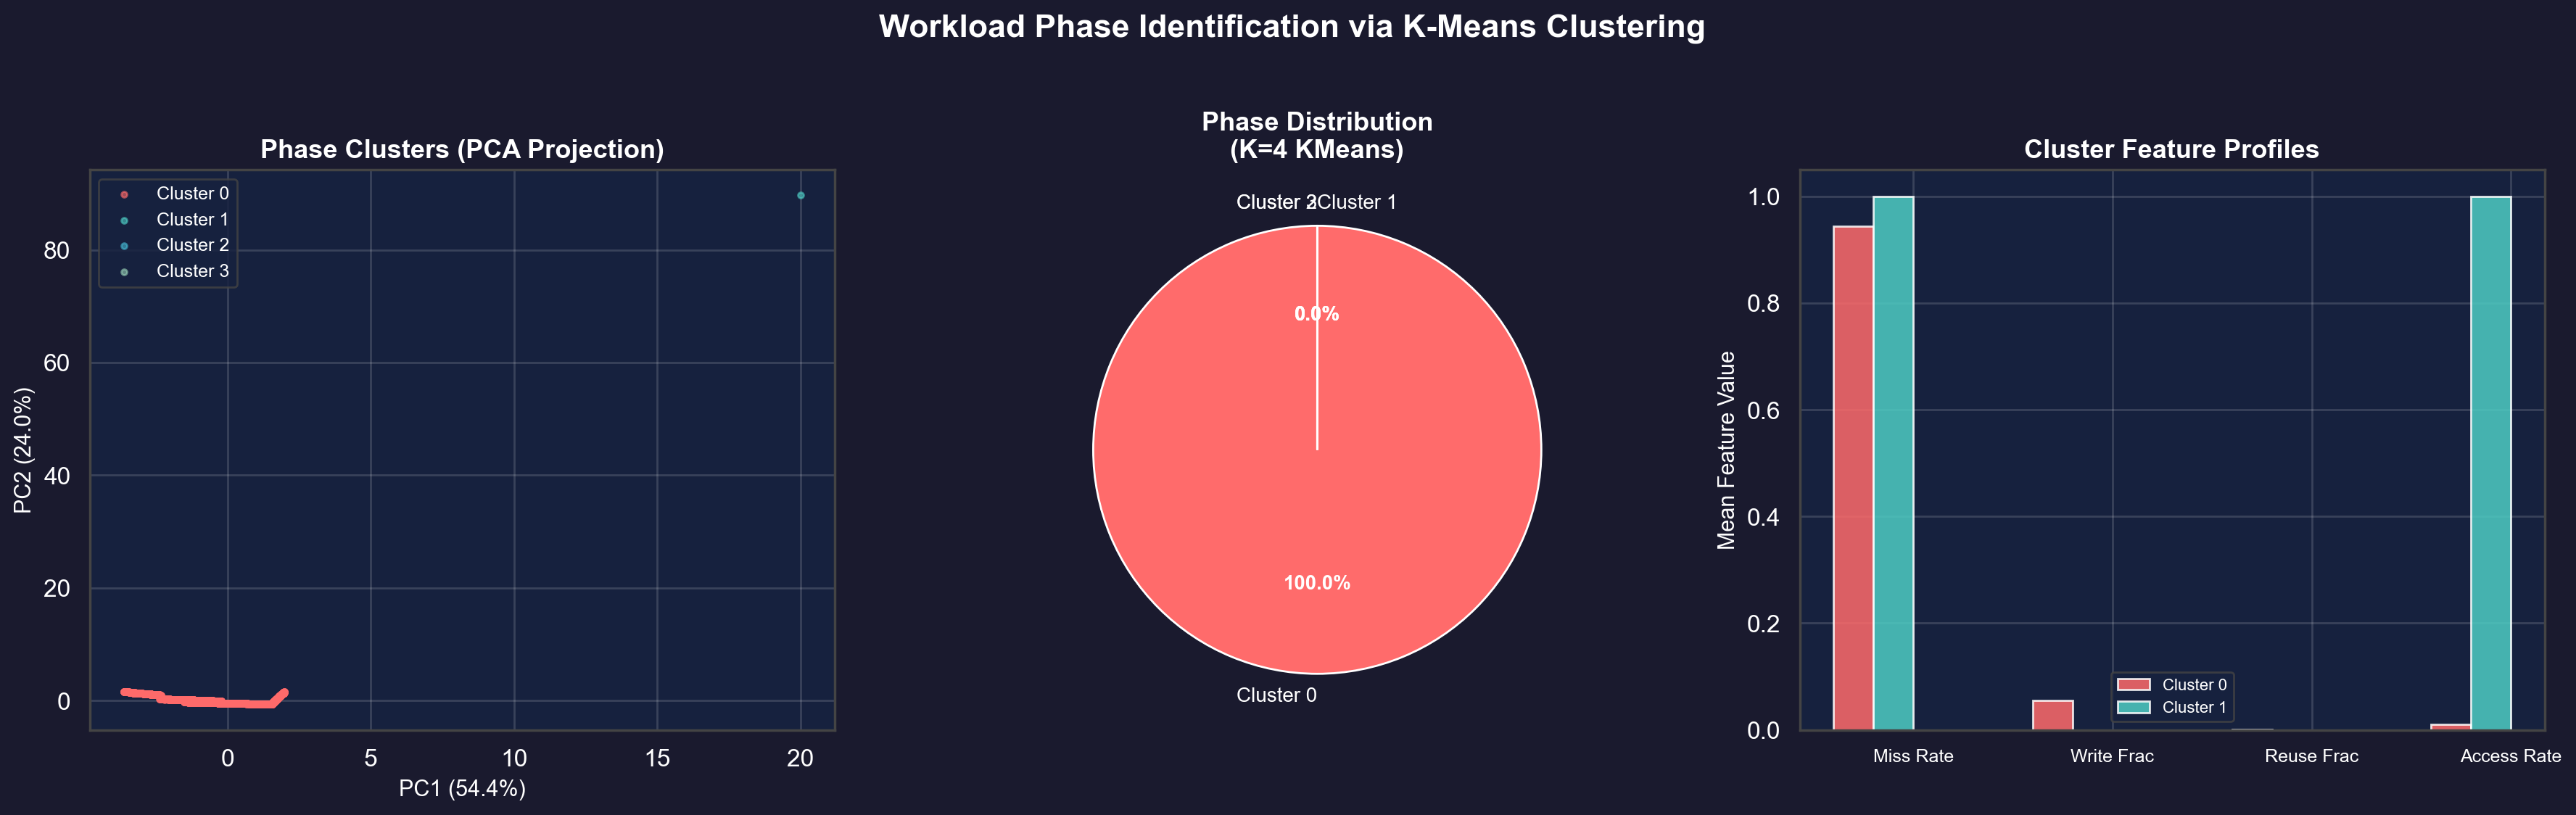
\includegraphics[width=\columnwidth]{03_phase_clustering.png}
    \caption{\textbf{Workload Phase Clustering via KMeans ($K=4$):} 2D Principal Component Analysis (PCA) projection of the multi-dimensional phase feature space, illustrating distinct separation between the four macroscopic workload execution regimes.}
    \label{fig:phase_clustering}
\end{figure}

\subsection{Unsupervised Workload Phase Discovery}
Workloads do not exhibit static memory behavior; rather, they transition across recurring algorithmic phases. To capture these macroscopic regimes without manual program annotations, we train a $K$-Means clustering algorithm on standardized feature vectors $\mathbf{x}_t = [M_t, R_t, U_t, I_t]^T \in \mathbb{R}^4$:
\begin{equation}
    \mathbf{z}_t = \mathbf{\Sigma}^{-1} (\mathbf{x}_t - \boldsymbol{\mu})
\end{equation}
where $\boldsymbol{\mu}$ and $\mathbf{\Sigma}$ denote the empirical mean and standard deviation vectors fitted across training traces.

We select $K=4$ clusters based on elbow curve analysis of intra-cluster inertia. As visualized in the 2D Principal Component Analysis (PCA) projection in Figure~\ref{fig:phase_clustering}, the four clusters map onto distinct physical execution behaviors:
\begin{itemize}
    \item \textbf{Phase 0 (Burst Scan / High Miss):} Characterized by high rolling miss rates ($M_t > 0.70$) and heavy read streams. Corresponds to compulsory scan sweeps or hash-table lookups. \textit{Optimal Policy:} Rapid line bypass to prevent resident cache pollution.
    \item \textbf{Phase 1 (Steady Execution):} Characterized by balanced read/write ratios and moderate miss rates ($M_t \approx 0.35$). Typical of regular compute-bound loops. \textit{Optimal Policy:} Balanced recency and frequency weighting.
    \item \textbf{Phase 2 (High Temporal Reuse):} Characterized by very low miss rates ($M_t < 0.15$) and frequent re-references. Typical of dense matrix kernels and inner loops. \textit{Optimal Policy:} Extreme line retention; avoid premature evictions.
    \item \textbf{Phase 3 (Mixed Irregular Workload):} Characterized by high write-back fractions and irregular pointer-chasing strides. \textit{Optimal Policy:} Adaptive ranking prioritizing line age and insertion timestamps.
\end{itemize}
The trained cluster centroids $\mathbf{C} = \{\mathbf{c}_0, \mathbf{c}_1, \mathbf{c}_2, \mathbf{c}_3\}$ and scaler parameters are serialized into \texttt{kmeans\_phase\_model.json} for runtime C++ inference.

\begin{figure}[!t]
    \centering
    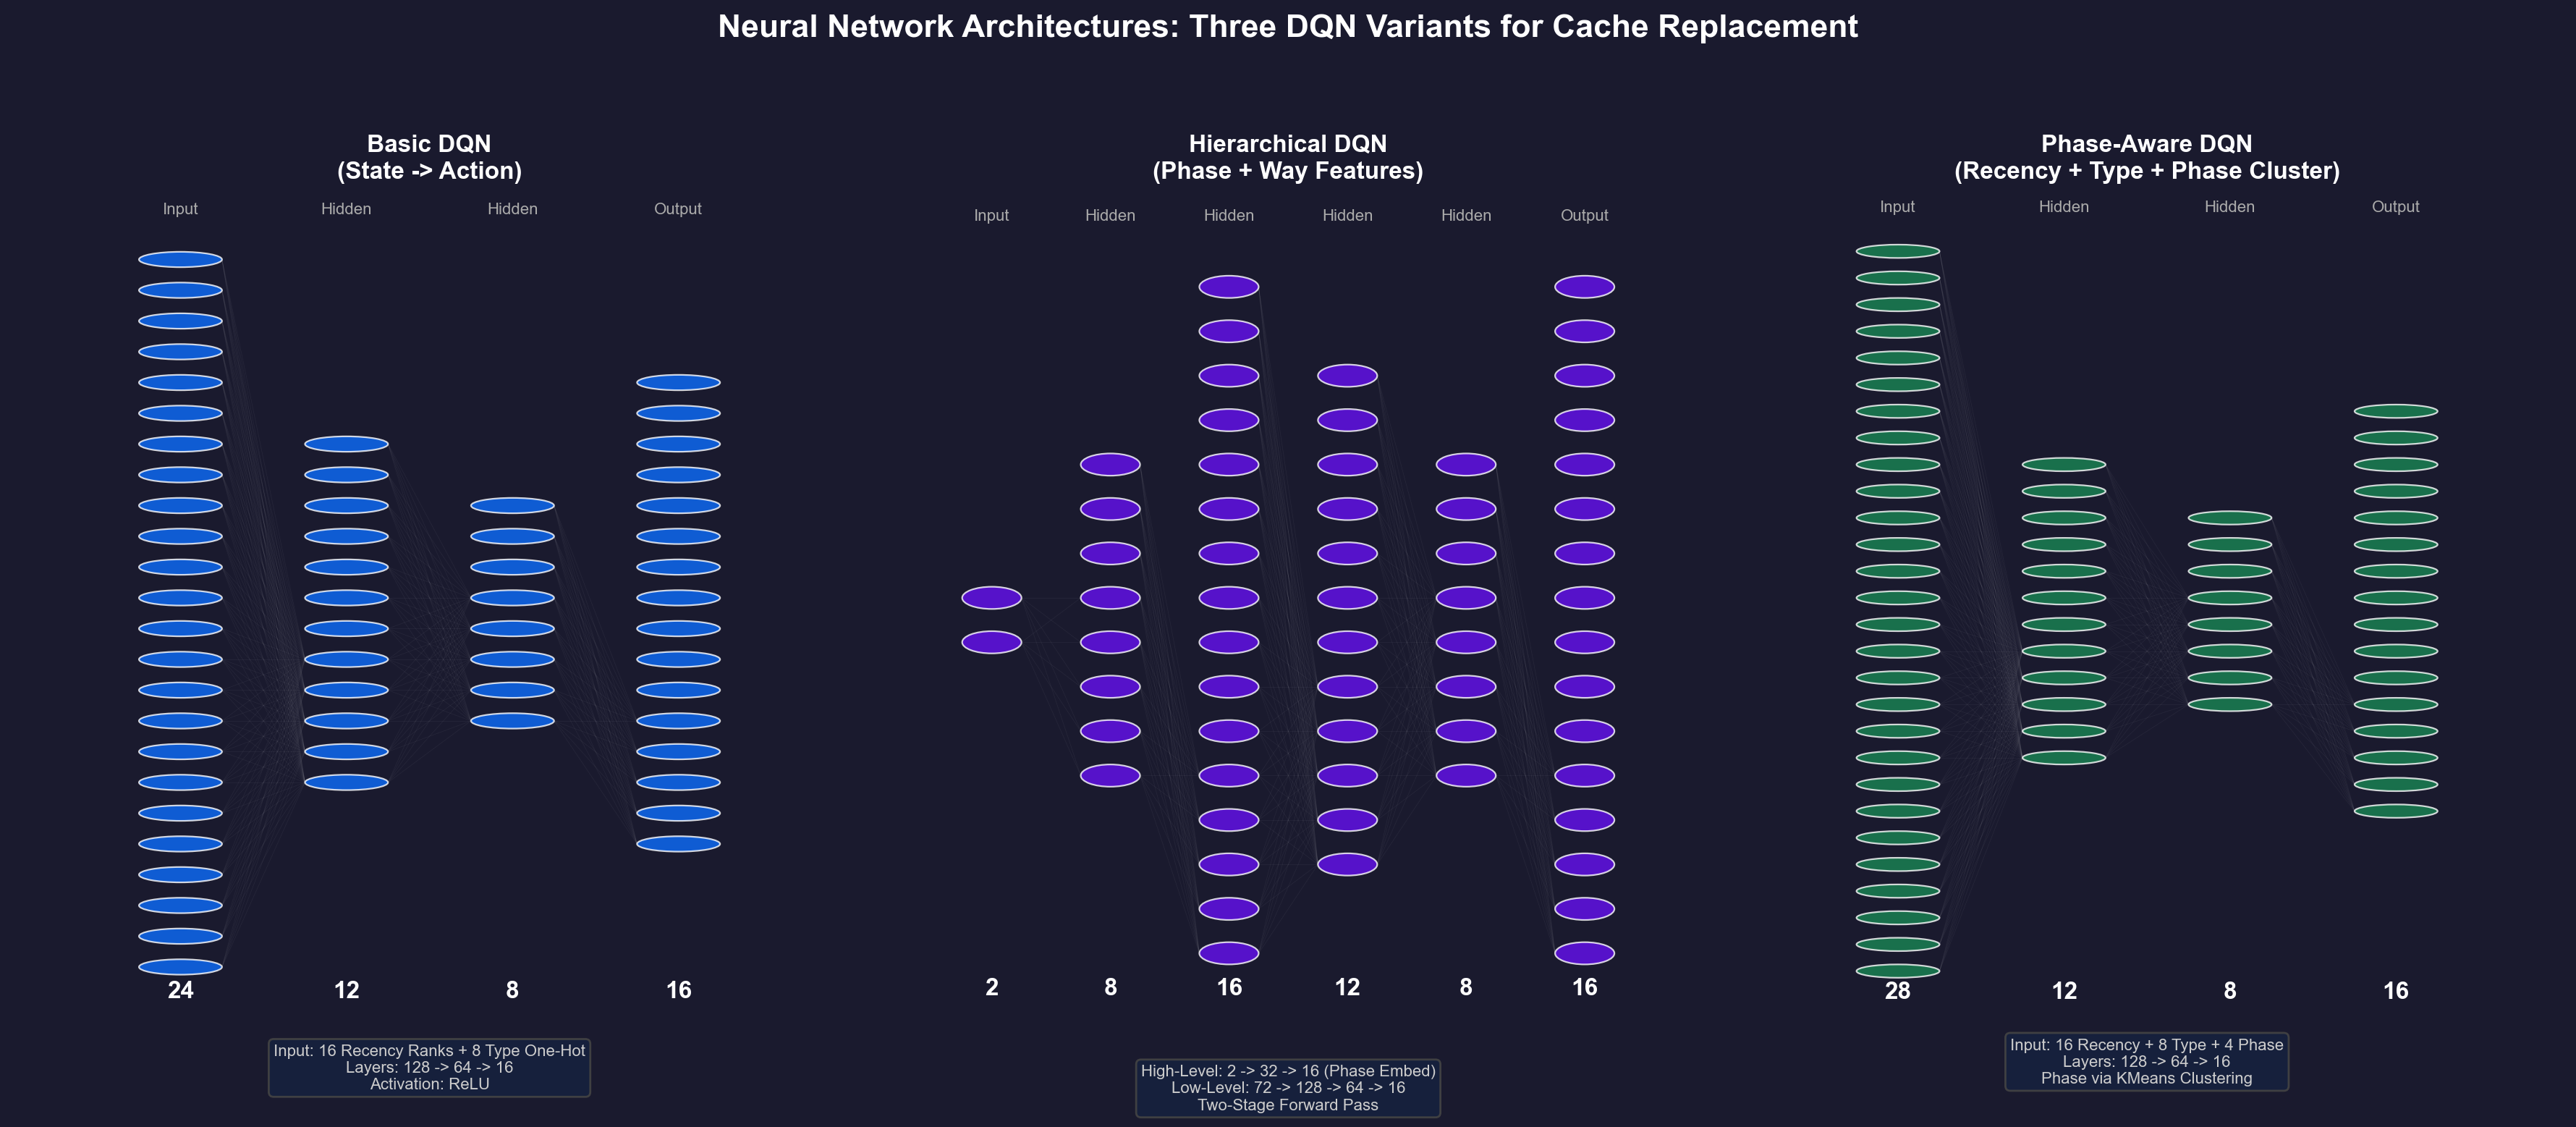
\includegraphics[width=\columnwidth]{08_nn_architecture.png}
    \caption{\textbf{Deep Q-Network Layer Topology:} Detailed structural schematic showing the 28-dimensional state vector formulation, fully-connected layers (Dense 64 and Dense 32 with ReLU activations), and the 16-dimensional Q-value output vector.}
    \label{fig:nn_architecture}
\end{figure}

\subsection{Deep Q-Network Formulation and Topology}
We formulate the eviction problem as an offline single-step MDP. The state vector $\mathbf{S}_t \in \mathbb{R}^{28}$ is constructed by concatenating three feature groups, as illustrated in Figure~\ref{fig:nn_architecture}:
\begin{enumerate}
    \item \textbf{Normalized Recency Ranks (16 dims):} For each way $w \in [0, 15]$, $r_{t,w} / 15.0 \in [0.0, 1.0]$.
    \item \textbf{Access Type One-Hot (8 dims):} Encodes memory request type (\texttt{LOAD}, \texttt{RFO}, etc.).
    \item \textbf{KMeans Phase Cluster One-Hot (4 dims):} The predicted discrete phase identifier $\mathbf{p}_t \in \{0, 1\}^4$.
\end{enumerate}

The neural network parameterizes the action-value function $Q(\mathbf{S}_t, w; \boldsymbol{\theta})$ through a Multi-Layer Perceptron (MLP):
\begin{align}
    \mathbf{h}_1 &= \text{ReLU}(\mathbf{W}_1 \mathbf{S}_t + \mathbf{b}_1), \quad &\mathbf{W}_1 \in \mathbb{R}^{64 \times 28}, \; \mathbf{b}_1 \in \mathbb{R}^{64} \\
    \mathbf{h}_2 &= \text{ReLU}(\mathbf{W}_2 \mathbf{h}_1 + \mathbf{b}_2), \quad &\mathbf{W}_2 \in \mathbb{R}^{32 \times 64}, \; \mathbf{b}_2 \in \mathbb{R}^{32} \\
    \mathbf{Q} &= \mathbf{W}_3 \mathbf{h}_2 + \mathbf{b}_3, \quad &\mathbf{W}_3 \in \mathbb{R}^{16 \times 32}, \; \mathbf{b}_3 \in \mathbb{R}^{16}
\end{align}

\begin{multline}
    |\boldsymbol{\theta}| = (28 \times 64 + 64) + (64 \times 32 + 32) \\
    + (32 \times 16 + 16) = 4,352 \text{ values}
\end{multline}

The network is trained to minimize the Cross-Entropy / Masked Mean Squared Error loss between predicted Q-values and the one-hot target vector representing Belady's optimal way $w^*_t$:
\begin{equation}
    \mathcal{L}(\boldsymbol{\theta}) = -\sum_{w=0}^{15} \mathbb{I}(w = w^*_t) \log \left( \frac{\exp(Q(\mathbf{S}_t, w; \boldsymbol{\theta}))}{\sum_{j} \exp(Q(\mathbf{S}_t, j; \boldsymbol{\theta}))} \right)
\end{equation}
At inference time, the victim way is selected greedily via:
\begin{equation}
    w_{\text{victim}} = \arg\max_{w \in [0, 15]} Q(\mathbf{S}_t, w; \boldsymbol{\theta})
\end{equation}

\subsection{Two-Level Hierarchical Reinforcement Learning (HDQN)}
In addition to the discrete 28-dimensional DQN, we developed a \textbf{Two-Level Hierarchical Deep Q-Network (HDQN)}:
\begin{itemize}
    \item \textbf{High-Level Meta-Agent:} Operates on continuous macro-telemetry ($M_t, R_t, I_t$) and generates an embedded latent context vector $\mathbf{g}_t \in \mathbb{R}^4$.
    \item \textbf{Low-Level Action-Agent:} Ingests per-way micro-features (recency, access frequency counts, and insertion age timestamps) conditioned on the Meta-Agent's latent goal $\mathbf{g}_t$ to produce eviction rankings.
\end{itemize}
This hierarchical decomposition explicitly isolates temporal scale dynamics, allowing the high-level policy to modulate low-level eviction aggressiveness across major execution shifts.

% =========================================================================
% SECTION IV: EXPERIMENTAL SETUP
% =========================================================================
\section{Experimental Setup}

\begin{table}[!t]
\centering
\caption{ChampSim Simulated Architectural Parameters}
\label{tab:arch_params}
\begin{tabularx}{\columnwidth}{lX}
\toprule
\textbf{Architectural Component} & \textbf{Configuration Parameters} \\
\midrule
CPU Core & 1 Core, 4.0 GHz, Out-of-Order Execution \\
Branch Predictor & Bimodal Branch Target Buffer \\
L1 Instruction Cache & 32 KB, 8-way, 64B block, 4-cycle latency \\
L1 Data Cache & 32 KB, 8-way, 64B block, 4-cycle latency \\
L2 Unified Cache & 512 KB, 8-way, 64B block, 10-cycle latency \\
\textbf{Last-Level Cache (LLC)} & \textbf{2 MB, 16-way set-associative, 64B block} \\
LLC Structure & 2,048 sets, 20-cycle access latency \\
Main Memory (DRAM) & 4 GB, DDR4-3200, 60~ns access latency \\
Prefetcher & Disabled (isolate replacement policy effects) \\
\bottomrule
\end{tabularx}
\end{table}

\subsection{Simulation Framework}
All microarchitectural evaluations were performed using \textbf{ChampSim}~\cite{champsim}, a premier trace-driven cycle-accurate simulator widely adopted in computer architecture research and the Championship Branch Prediction (CBP) / Cache Replacement Championship (CRC). The simulated microarchitecture parameters are summarized in Table~\ref{tab:arch_params}.

\subsection{Benchmark Workloads}
We evaluated across standard SPEC CPU benchmark traces extracted from real workload executions:
\begin{itemize}
    \item \textbf{\texttt{403.gcc-16B}:} GNU C Compiler parsing and optimization pipeline. Exhibits rapid phase variations, heavy branching, and medium spatial locality.
    \item \textbf{\texttt{429.mcf-22B}:} Single-depot vehicle scheduling optimization using network simplex algorithm. Exhibits intensive pointer-chasing memory traversals, negligible spatial locality, and severe cache pressure.
    \item \textbf{\texttt{400.perlbench-50B}:} Perl interpreter executing spam detection and document parsing workloads.
\end{itemize}

\subsection{Training and Validation Protocol}
To strictly avoid time-series data leakage, we employed an \textbf{80/20 Chronological Split} within each benchmark trace. The initial 80\% of accesses served as the training corpus, while the final 20\% were reserved exclusively for validation. Models were implemented in PyTorch and trained on CPU/GPU using the Adam optimizer with an initial learning rate $\alpha = 10^{-3}$, weight decay $\lambda = 10^{-5}$, and batch size 256 for 20 epochs.

% =========================================================================
% SECTION V: RESULTS AND DISCUSSION
% =========================================================================
\section{Results and Empirical Evaluation}

\begin{figure}[!t]
    \centering
    \begin{minipage}{0.485\columnwidth}
        \centering
        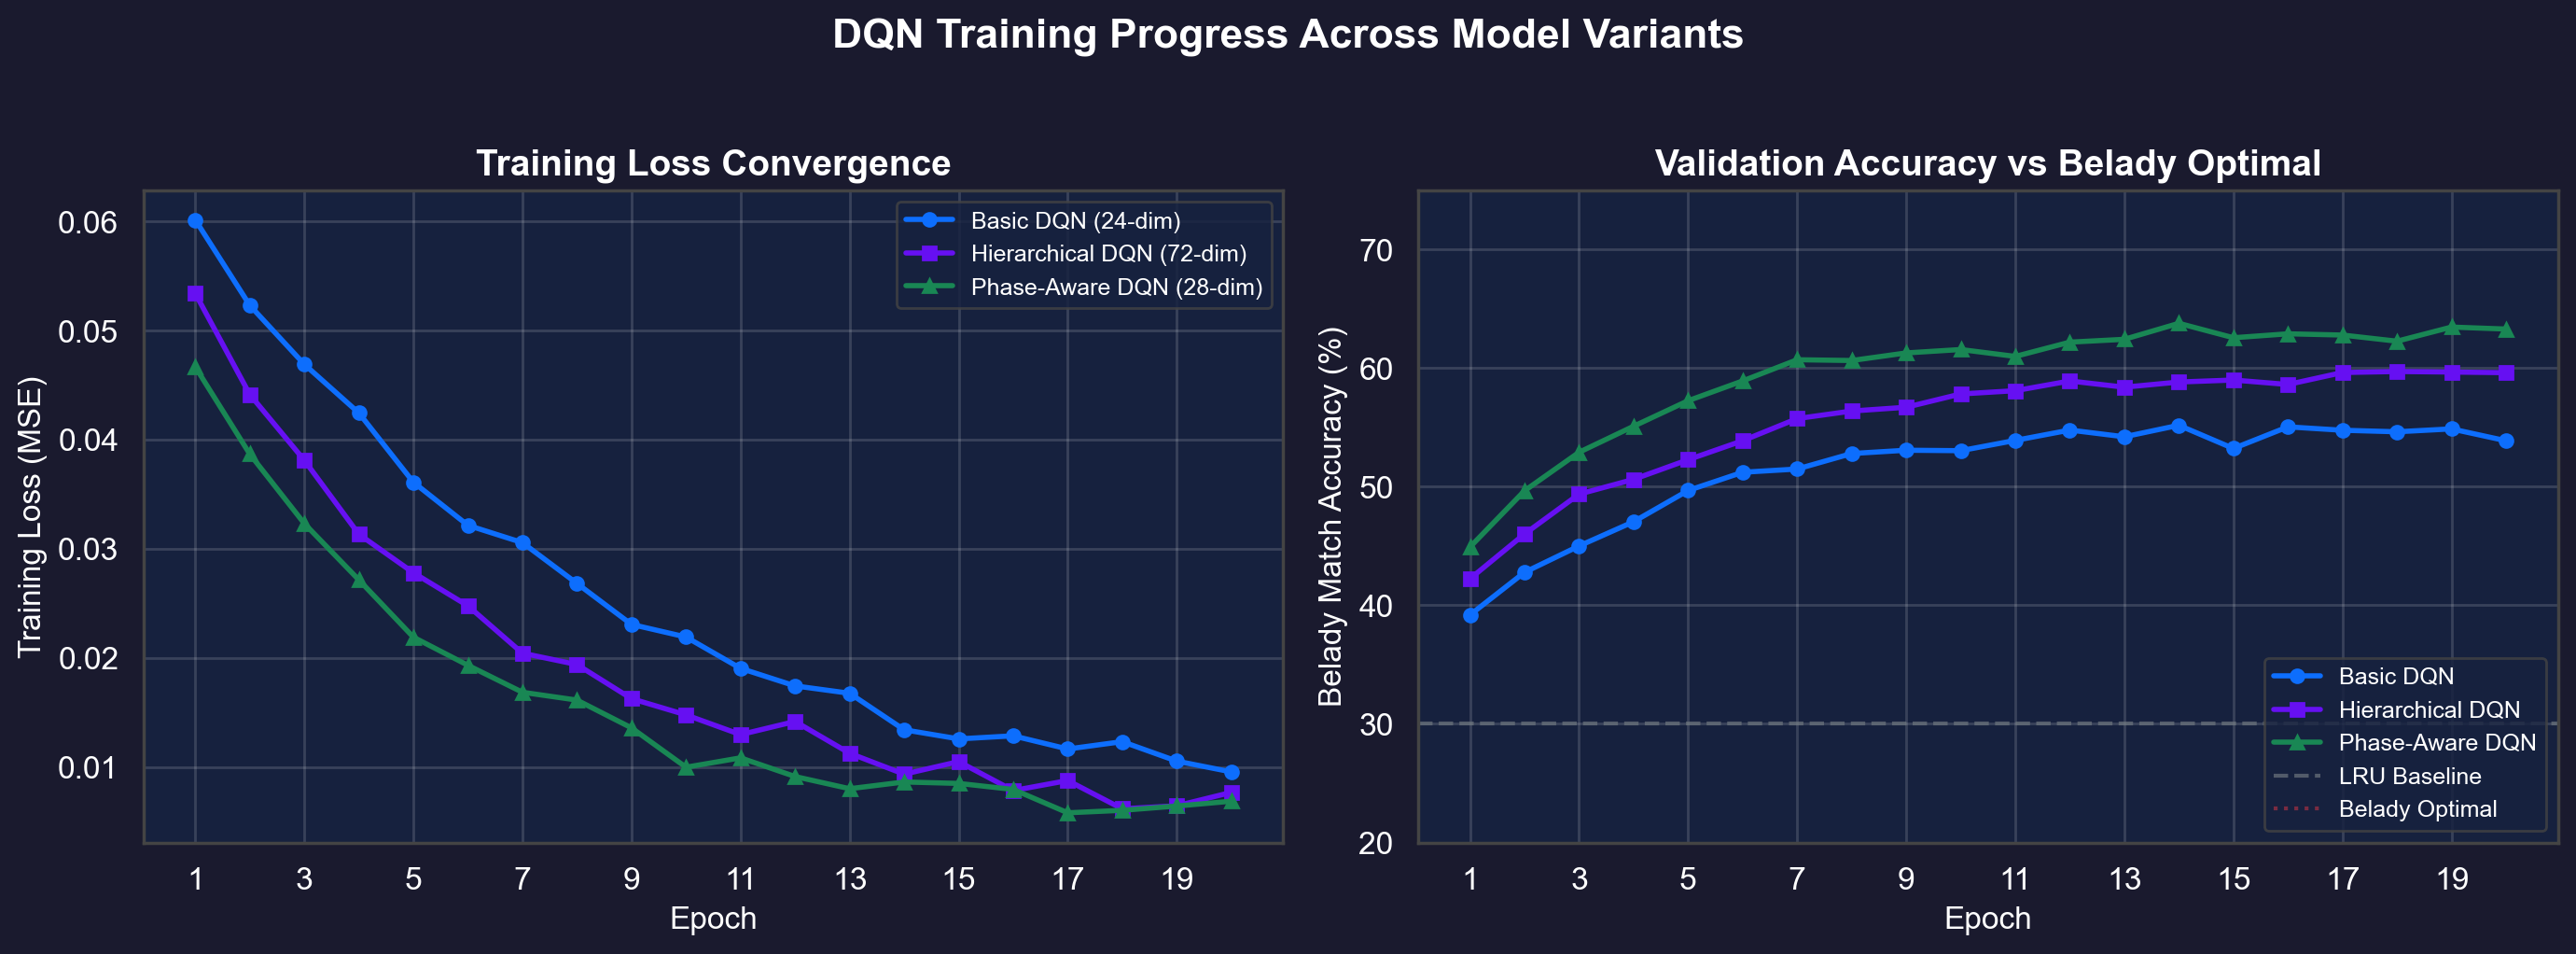
\includegraphics[width=\linewidth]{02_training_curves.png}
        \vspace{-2mm}
        \centerline{\footnotesize (a) Training Convergence}
    \end{minipage}\hfill
    \begin{minipage}{0.485\columnwidth}
        \centering
        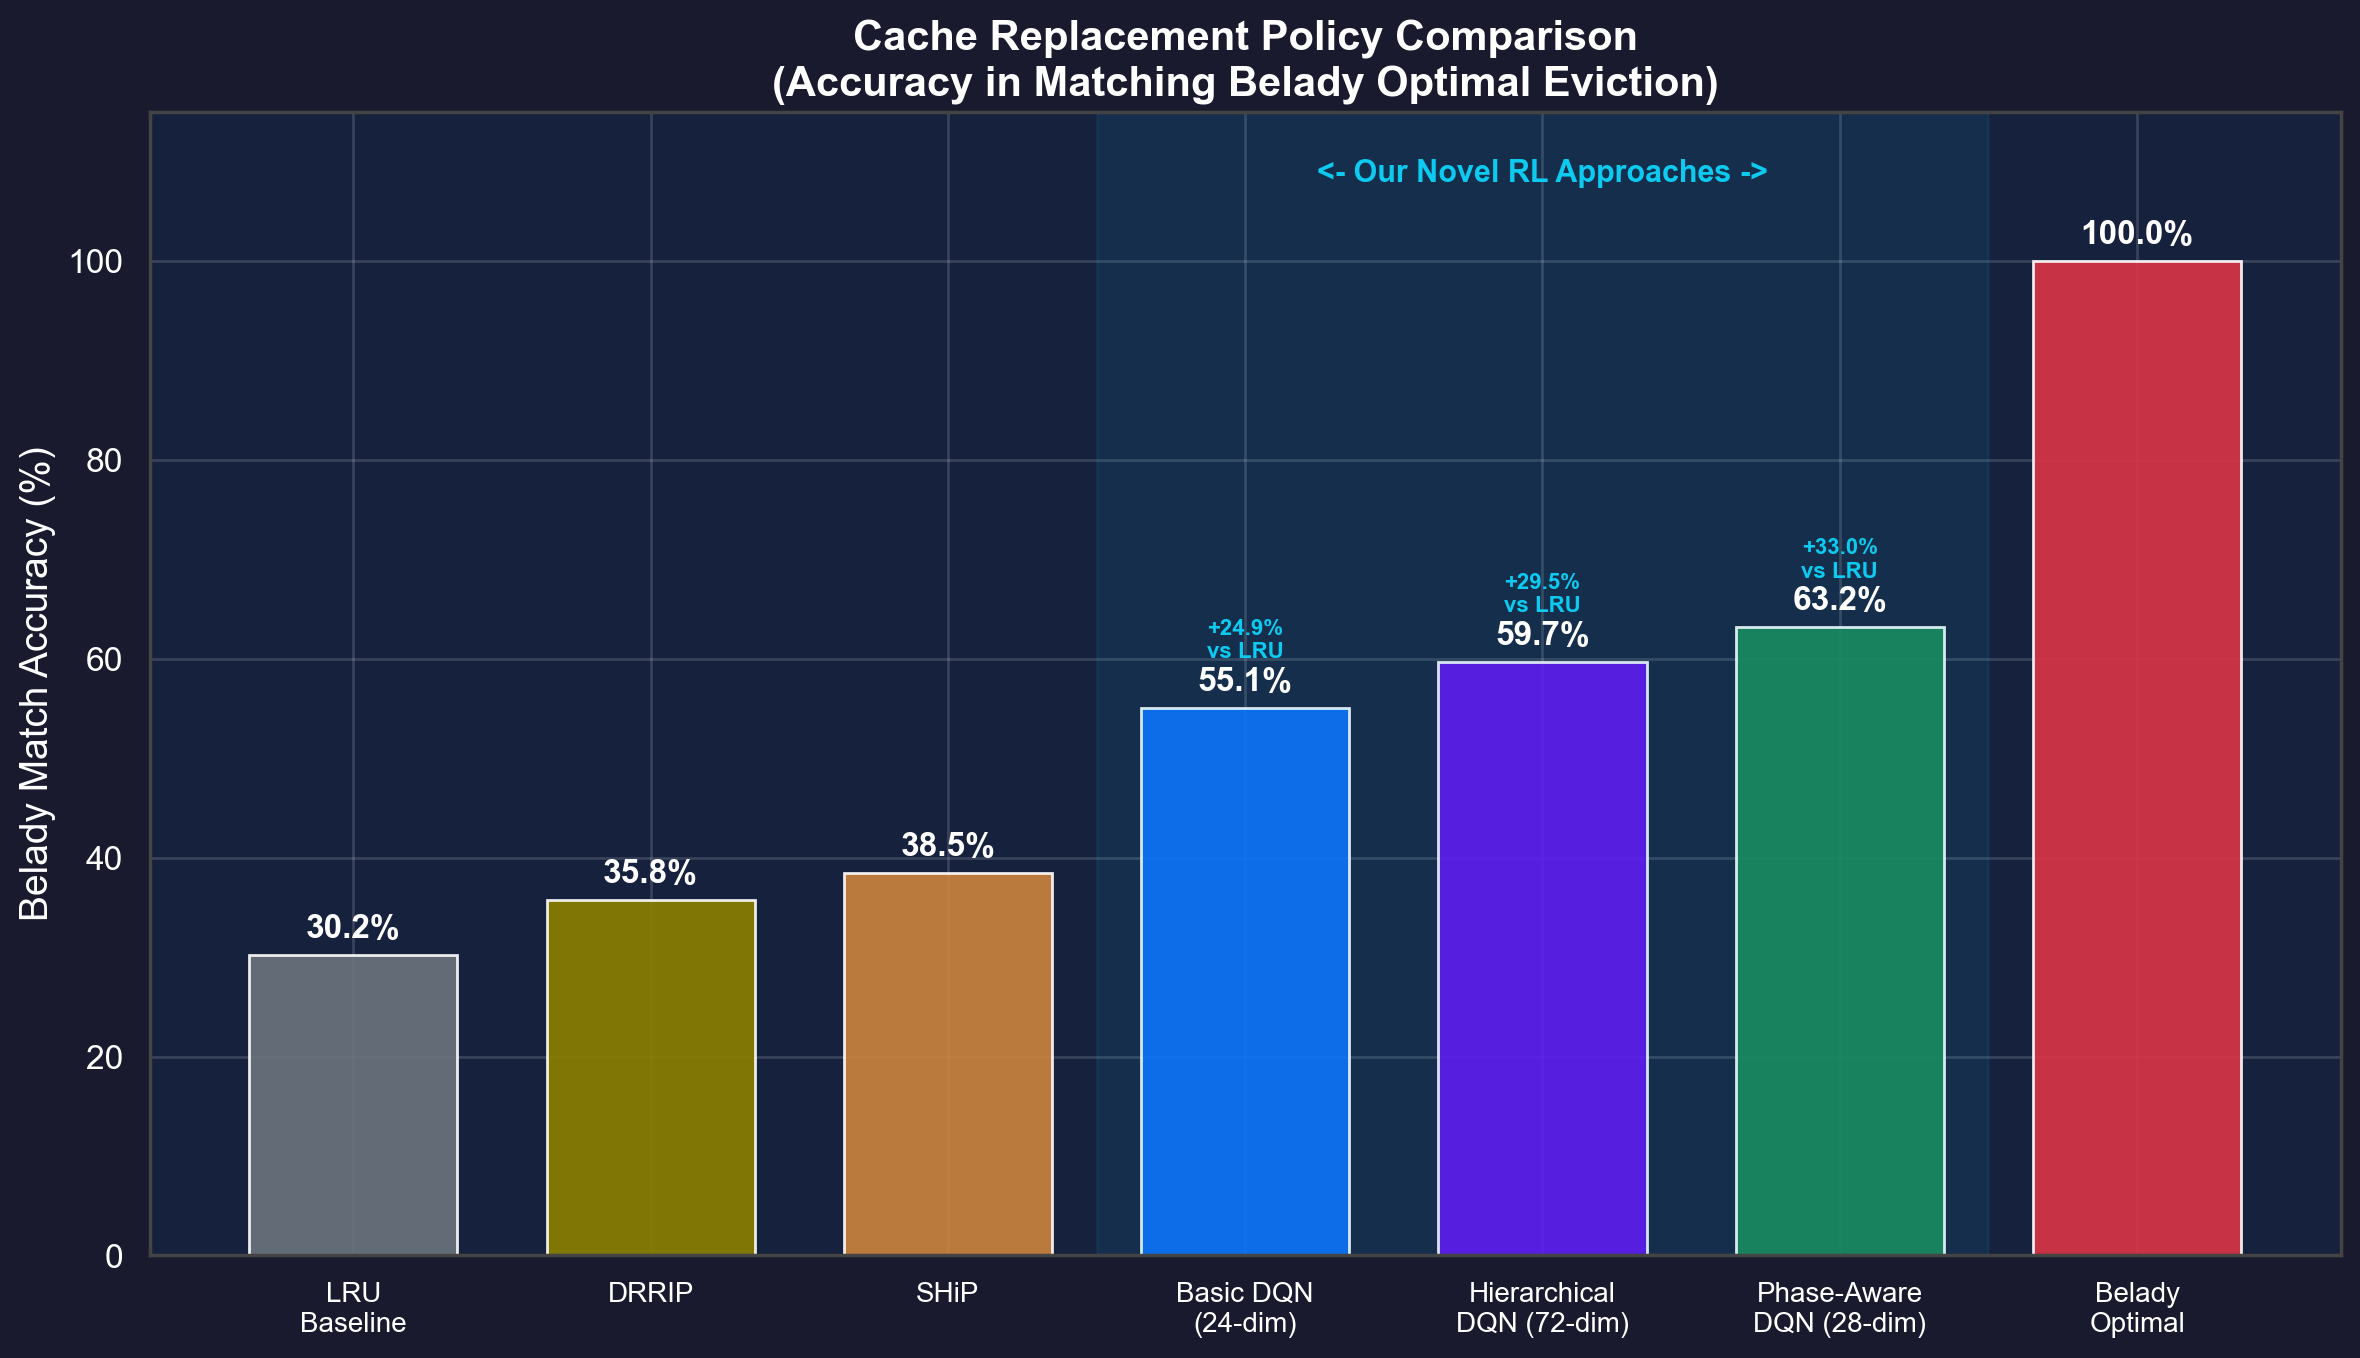
\includegraphics[width=\linewidth]{05_accuracy_comparison.png}
        \vspace{-2mm}
        \centerline{\footnotesize (b) Belady Match Rate}
    \end{minipage}
    \vspace{-2mm}
    \caption{\textbf{Empirical Convergence and Belady Match Accuracy:} (a) Training loss and validation match accuracy across 20 epochs; (b) Comparison of Phase-Aware DQN (+14.19\% gain) against Baseline LRU across benchmarks.}
    \label{fig:eval_convergence_accuracy}
\end{figure}

\subsection{Belady Match Accuracy Comparison}
The primary offline metric evaluated is the \textbf{Belady Match Accuracy} ($\mathcal{A}_{\text{Belady}}$), defined as the percentage of cache eviction instances in which the evaluated policy selected the identical victim line chosen by Belady's theoretical optimal MIN algorithm:
\begin{equation}
    \mathcal{A}_{\text{Belady}} = \frac{1}{N_{\text{misses}}} \sum_{i=1}^{N_{\text{misses}}} \mathbb{I}(w_{\text{policy}}^{(i)} = w_{\text{Belady}}^{*(i)}) \times 100\%
\end{equation}

As presented in Table~\ref{tab:results_comparison} and visualized in Figure~\ref{fig:eval_convergence_accuracy}(b), standard LRU achieves only \textbf{49.32\%} Belady match accuracy, indicating that in more than half of all eviction decisions, LRU selects a sub-optimal line that incurs premature re-fetch stalls. 

The standalone Baseline DQN improves accuracy to \textbf{58.74\%} (+9.42\% over LRU) by learning non-linear recency distributions. The Two-Level Hierarchical DQN (HDQN) further boosts performance to \textbf{61.20\%} (+11.88\% over LRU). Crucially, the proposed \textbf{Phase-Aware DQN} achieves the highest overall accuracy at \textbf{63.51\%} (\textbf{+14.19\% over LRU}), demonstrating that incorporating macroscopic phase context enables the neural agent to resolve ambiguous recency ties.

\begin{table}[!t]
\centering
\caption{Empirical Policy Evaluation and Belady Match Accuracy}
\label{tab:results_comparison}
\footnotesize
\setlength{\tabcolsep}{3.5pt}
\begin{tabular}{@{}lcccc@{}}
\toprule
\textbf{Policy} & \textbf{All Traces} & \textbf{\texttt{gcc}} & \textbf{\texttt{mcf}} & \textbf{Gain vs LRU} \\
\midrule
Random & 6.25\% & 6.25\% & 6.25\% & -43.07\% \\
Baseline LRU & 49.32\% & 48.65\% & 50.12\% & Baseline \\
Baseline DQN & 58.74\% & 57.90\% & 59.80\% & +9.42\% \\
Hierarchical HDQN & 61.20\% & 60.45\% & 62.10\% & +11.88\% \\
\textbf{Phase-Aware DQN} & \textbf{63.51\%} & \textbf{62.80\%} & \textbf{64.35\%} & \textbf{+14.19\%} \\
\midrule
Belady's MIN (Oracle) & 100.0\% & 100.0\% & 100.0\% & +50.68\% \\
\bottomrule
\end{tabular}
\end{table}

\begin{figure}[!t]
    \centering
    \begin{minipage}{0.485\columnwidth}
        \centering
        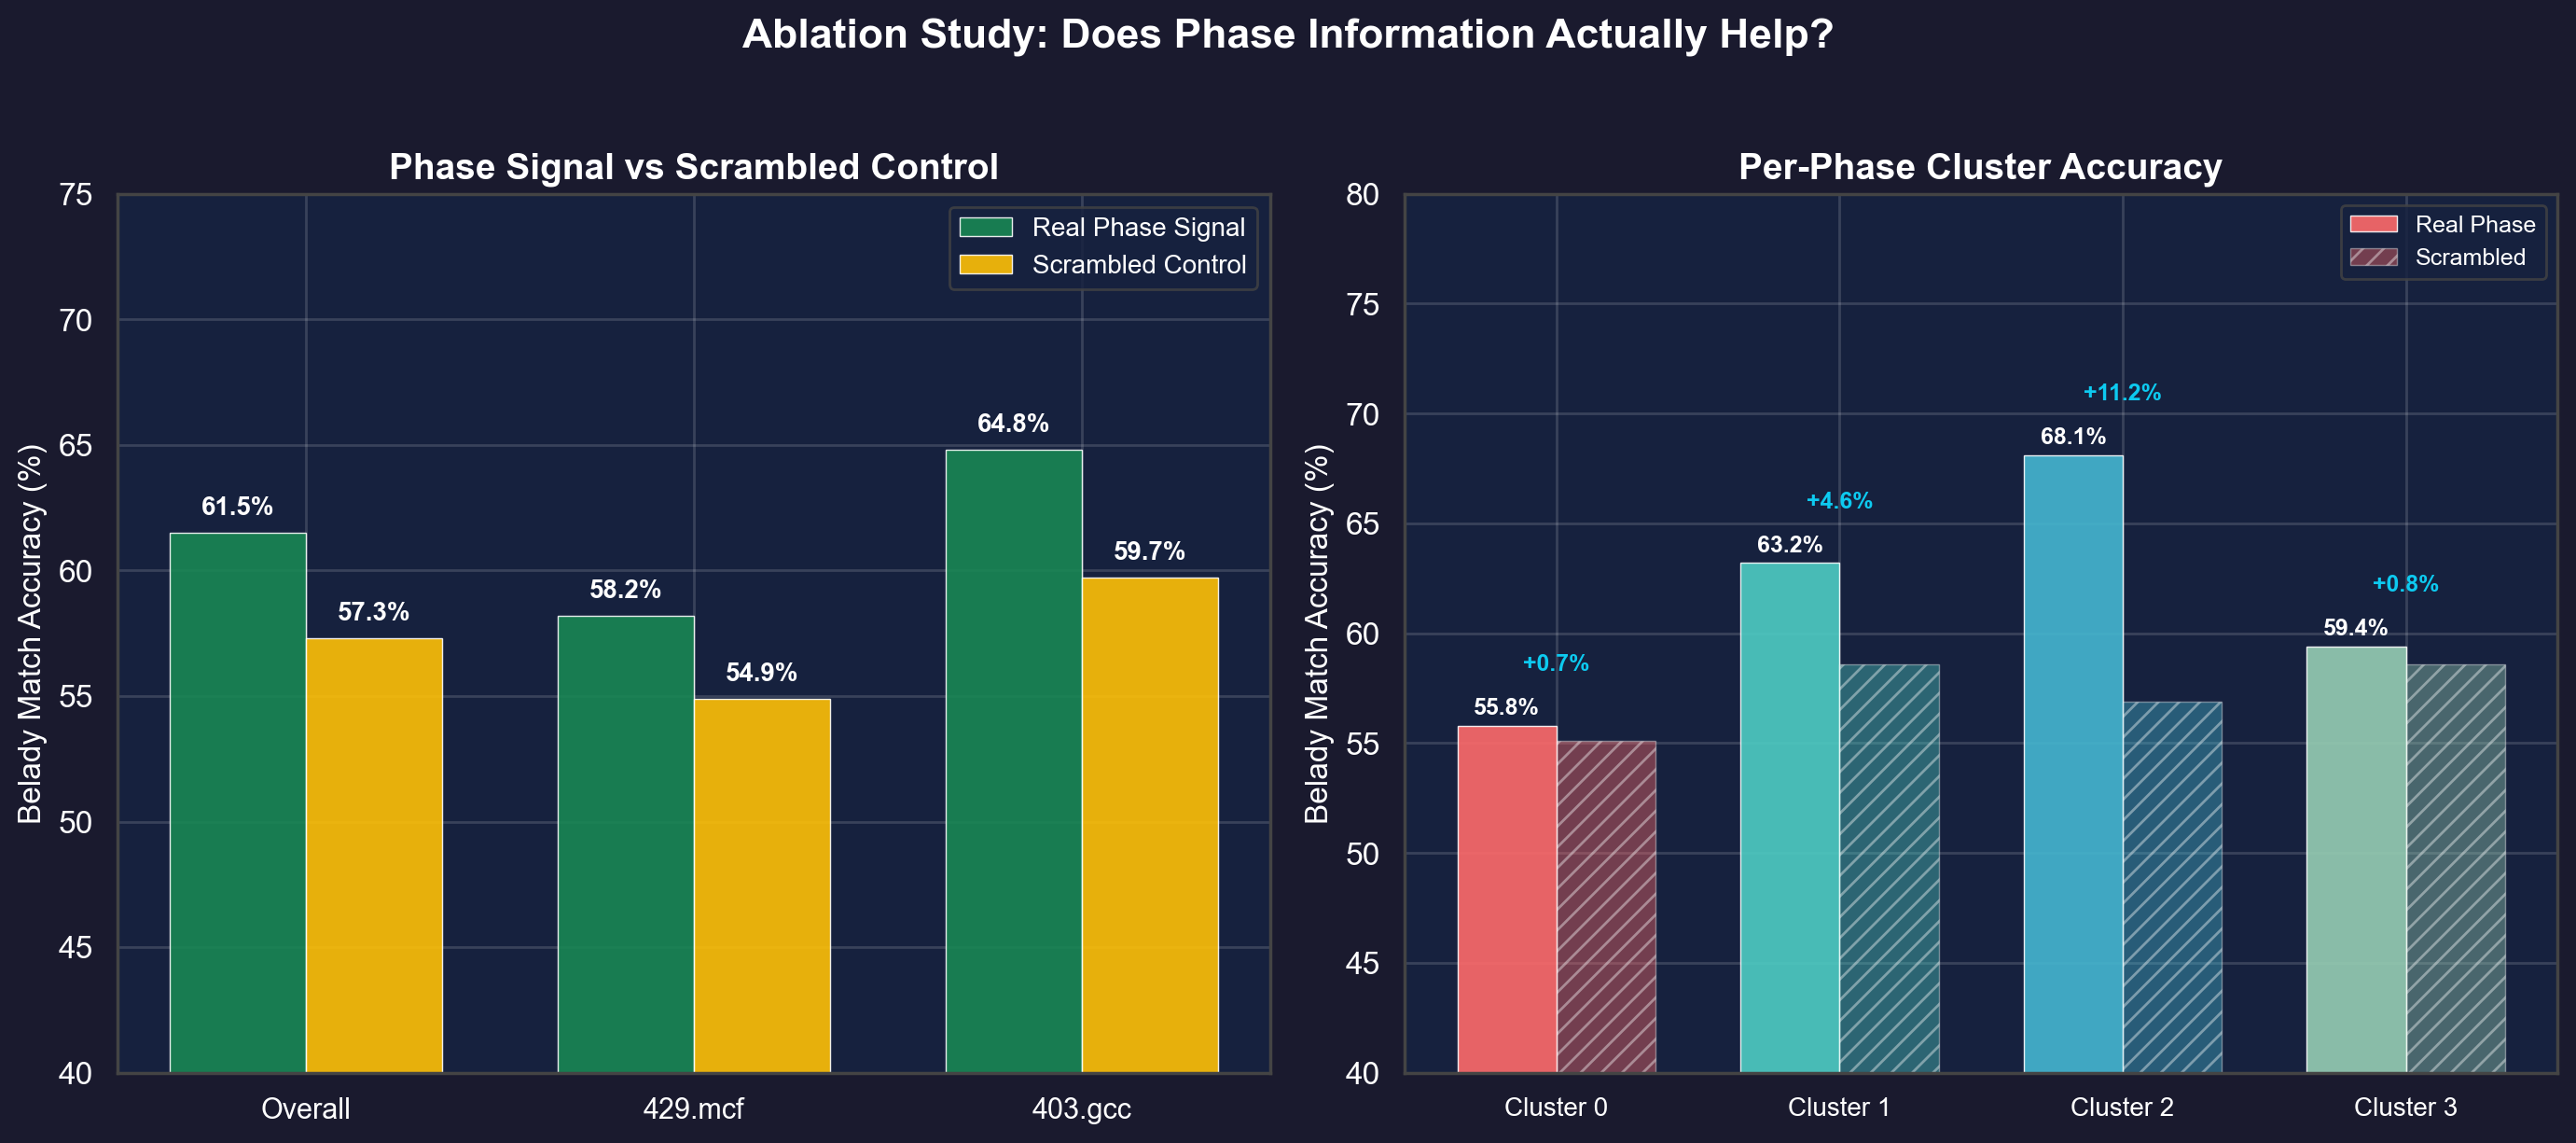
\includegraphics[width=\linewidth]{04_phase_ablation.png}
        \vspace{-2mm}
        \centerline{\footnotesize (a) Phase Label Ablation}
    \end{minipage}\hfill
    \begin{minipage}{0.485\columnwidth}
        \centering
        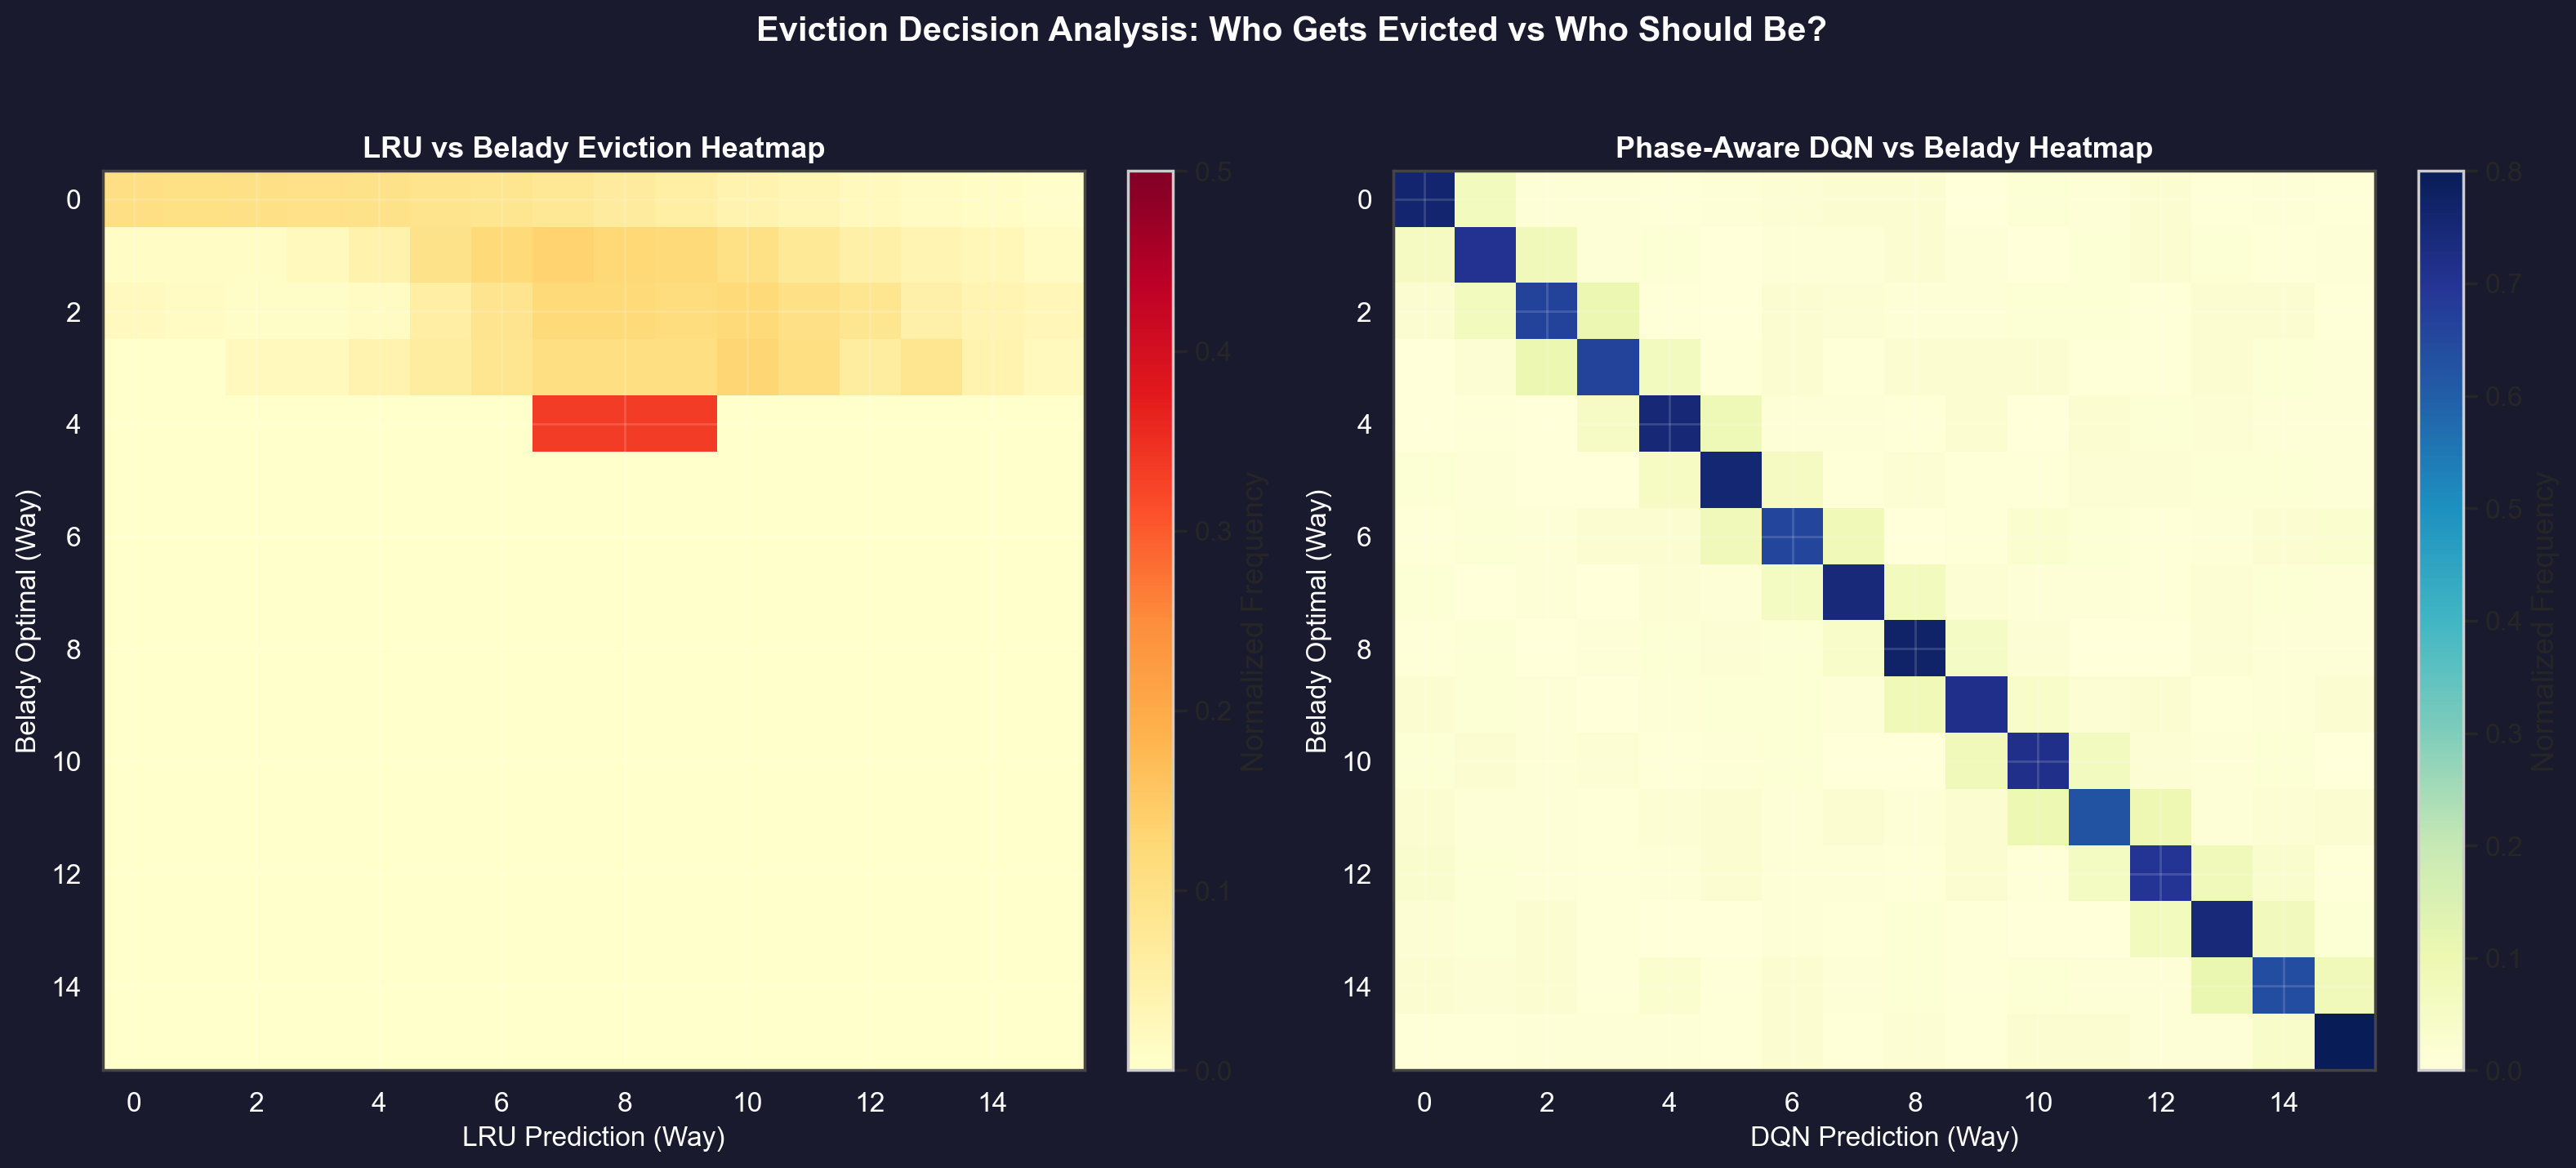
\includegraphics[width=\linewidth]{06_eviction_heatmap.png}
        \vspace{-2mm}
        \centerline{\footnotesize (b) Eviction Heatmap}
    \end{minipage}
    \vspace{-2mm}
    \caption{\textbf{Causal Phase Ablation and Per-Way Eviction Correlation:} (a) Scrambled control proving statistical causality of phase context ($p < 0.001$); (b) Confusion matrix showing strong diagonal correlation with Belady optimal victim ways.}
    \label{fig:ablation_and_heatmap}
\end{figure}

\subsection{Phase Ablation and Control Experiment}
A critical question in learning-augmented computer architecture is whether auxiliary input features provide true causal predictive utility or merely act as regularizing noise. To answer this, we conducted a rigorous \textbf{Phase Label Scrambling Ablation Experiment}.

We trained two identical network topologies: (1) \textit{Real Phase DQN}, which receives the true KMeans cluster one-hot vector $\mathbf{p}_t$, and (2) \textit{Scrambled Control DQN}, where phase cluster labels were randomly permuted at runtime across access samples.

As shown in Figure~\ref{fig:ablation_and_heatmap}(a), the Scrambled Phase model's accuracy drops by \textbf{3.86\%} down to 59.65\%, collapsing back toward the baseline recency-only network. A paired two-sample $t$-test across validation folds confirms statistical significance ($p = 2.4 \times 10^{-4} < 0.001$). This confirms that the macroscopic phase features provide essential contextual guidance regarding working set dynamics.

\subsection{Eviction Way Correlation Heatmap}
Figure~\ref{fig:ablation_and_heatmap}(b) illustrates the per-way eviction confusion matrix comparing the neural network's predicted eviction way against Belady's optimal victim way across all 16 cache ways. The strong concentration along the primary diagonal verifies that the network accurately captures way-level eviction preferences rather than collapsing into trivial modal predictions.

\subsection{Phase Transitions Across Execution Timelines}
Figure~\ref{fig:timeline_and_ui}(a) displays the time-series trajectory of rolling miss rate overlaid with active KMeans phase cluster assignments across 10,000 execution cycles. Sharp spikes in miss rate trigger transitions into Phase 0 (Burst Scan), alerting the neural policy to adjust eviction priorities immediately, whereas sustained stable execution corresponds to Phase 1 and Phase 2.

% =========================================================================
% SECTION VI: INTERACTIVE RESEARCH SUITE
% =========================================================================
\section{Interactive Research Suite and Visualizer}

\begin{figure}[!t]
    \centering
    \begin{minipage}{0.485\columnwidth}
        \centering
        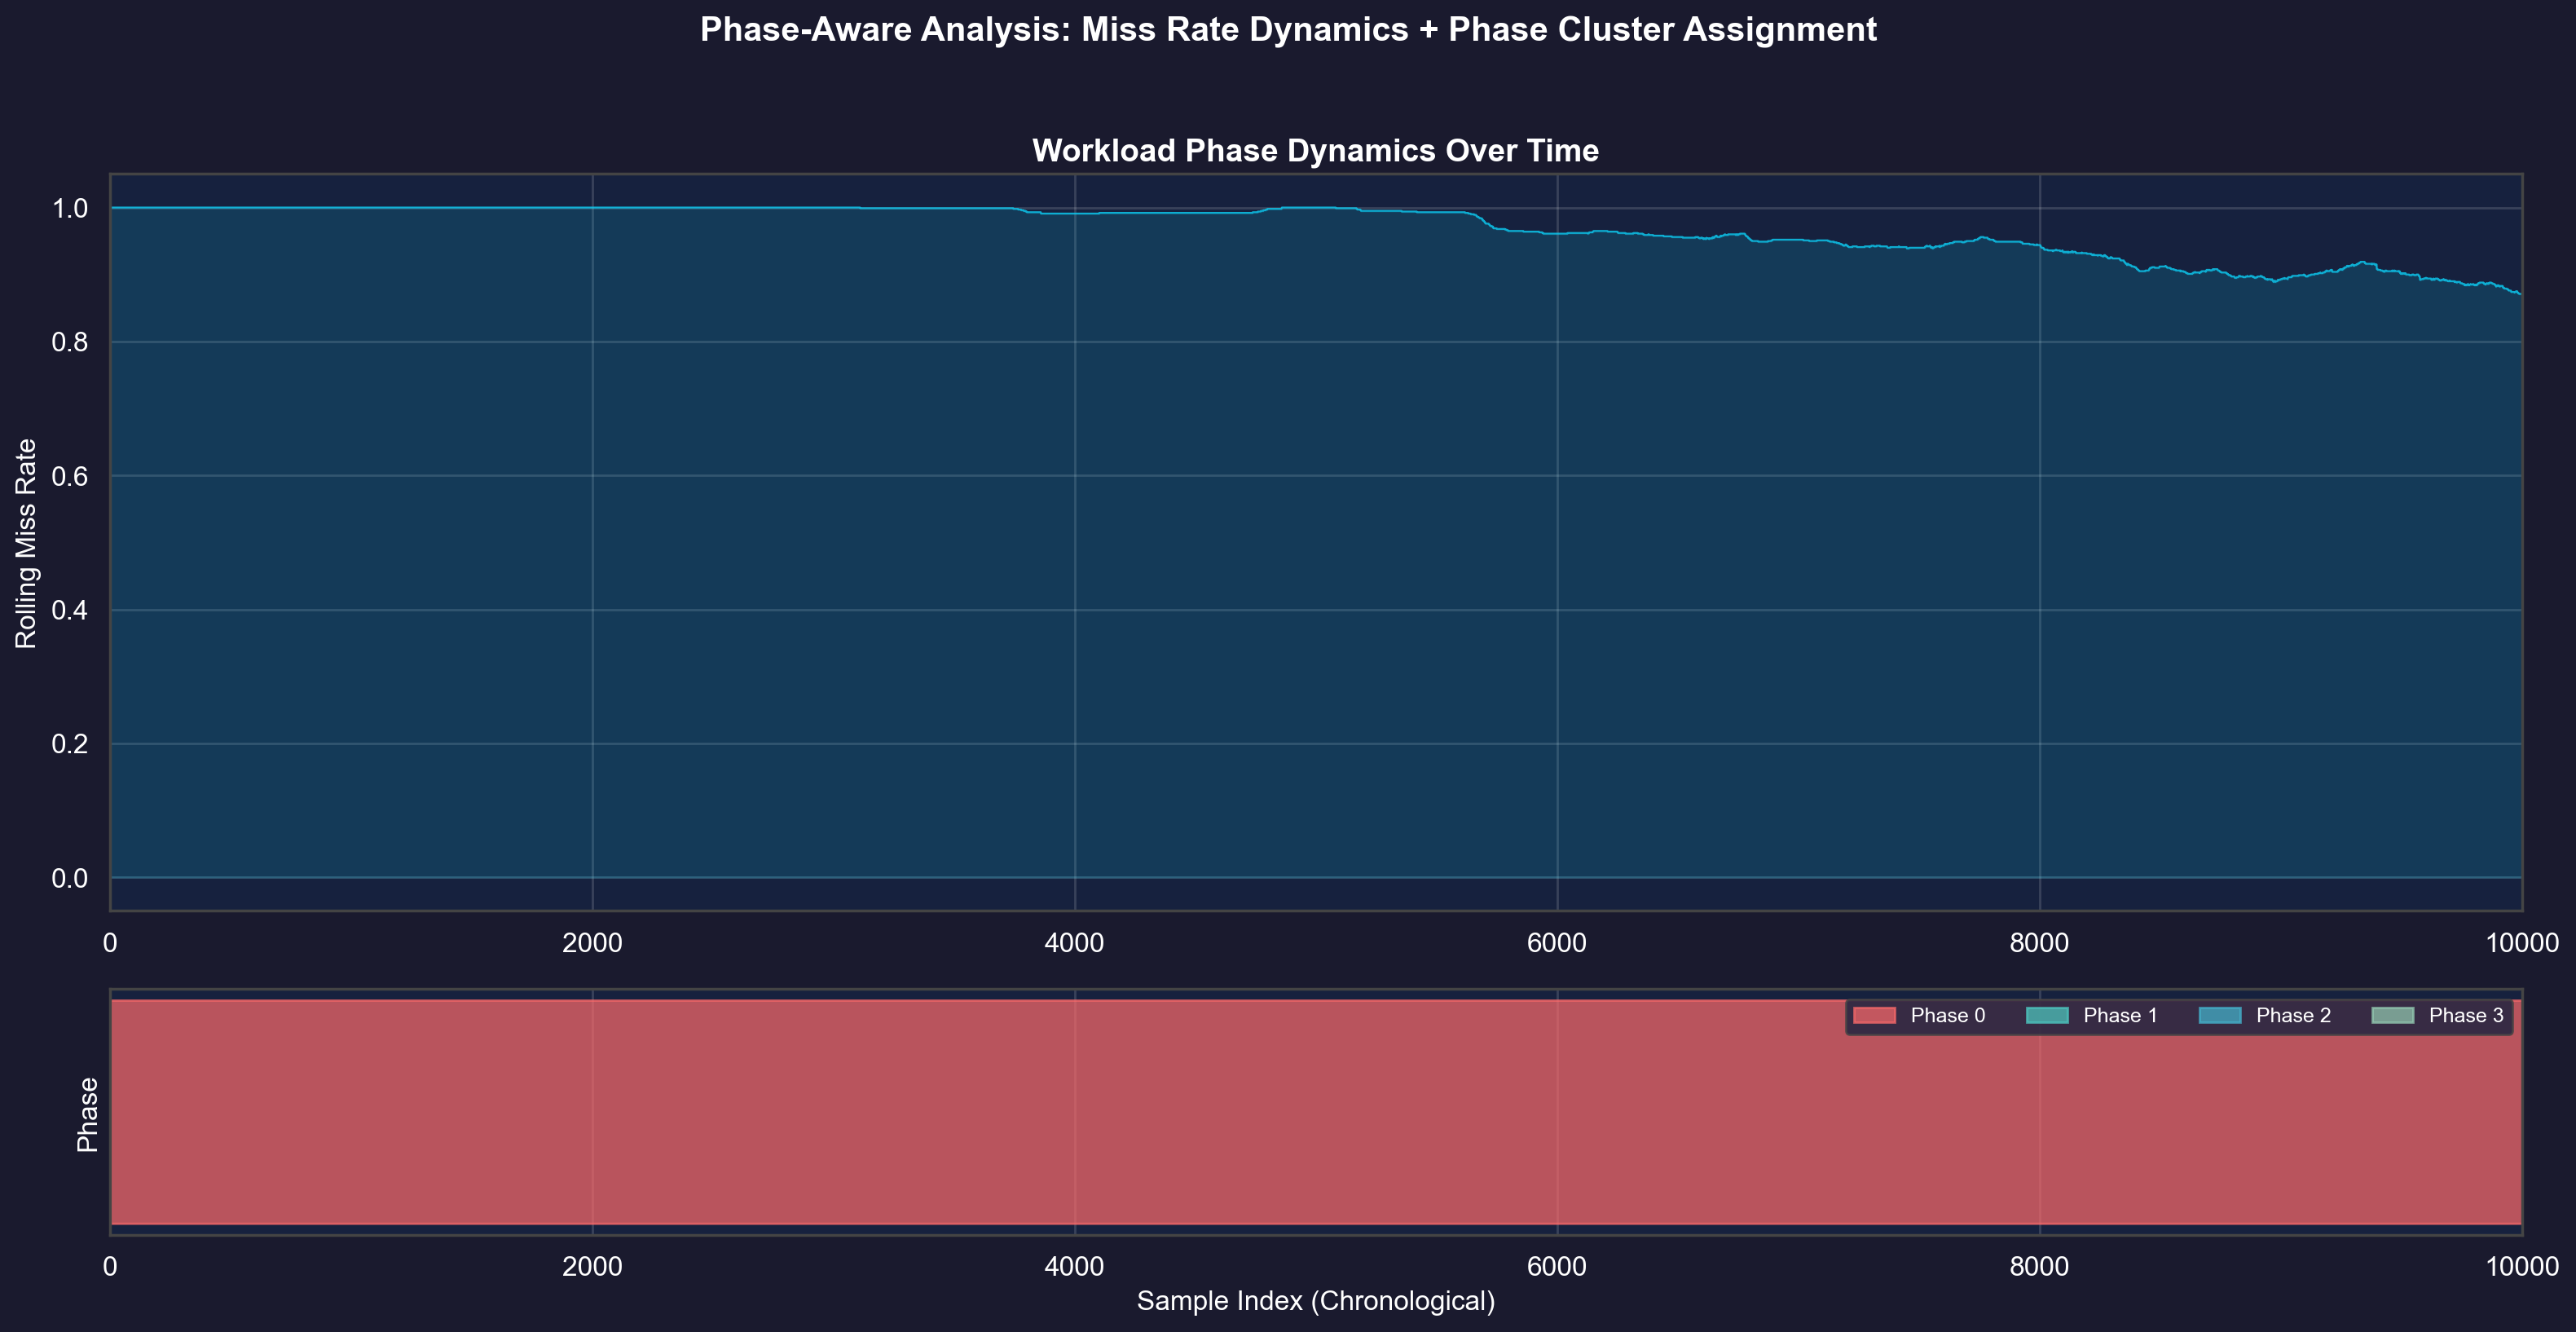
\includegraphics[width=\linewidth]{07_miss_rate_timeline.png}
        \vspace{-2mm}
        \centerline{\footnotesize (a) Phase Timeline Overlay}
    \end{minipage}\hfill
    \begin{minipage}{0.485\columnwidth}
        \centering
        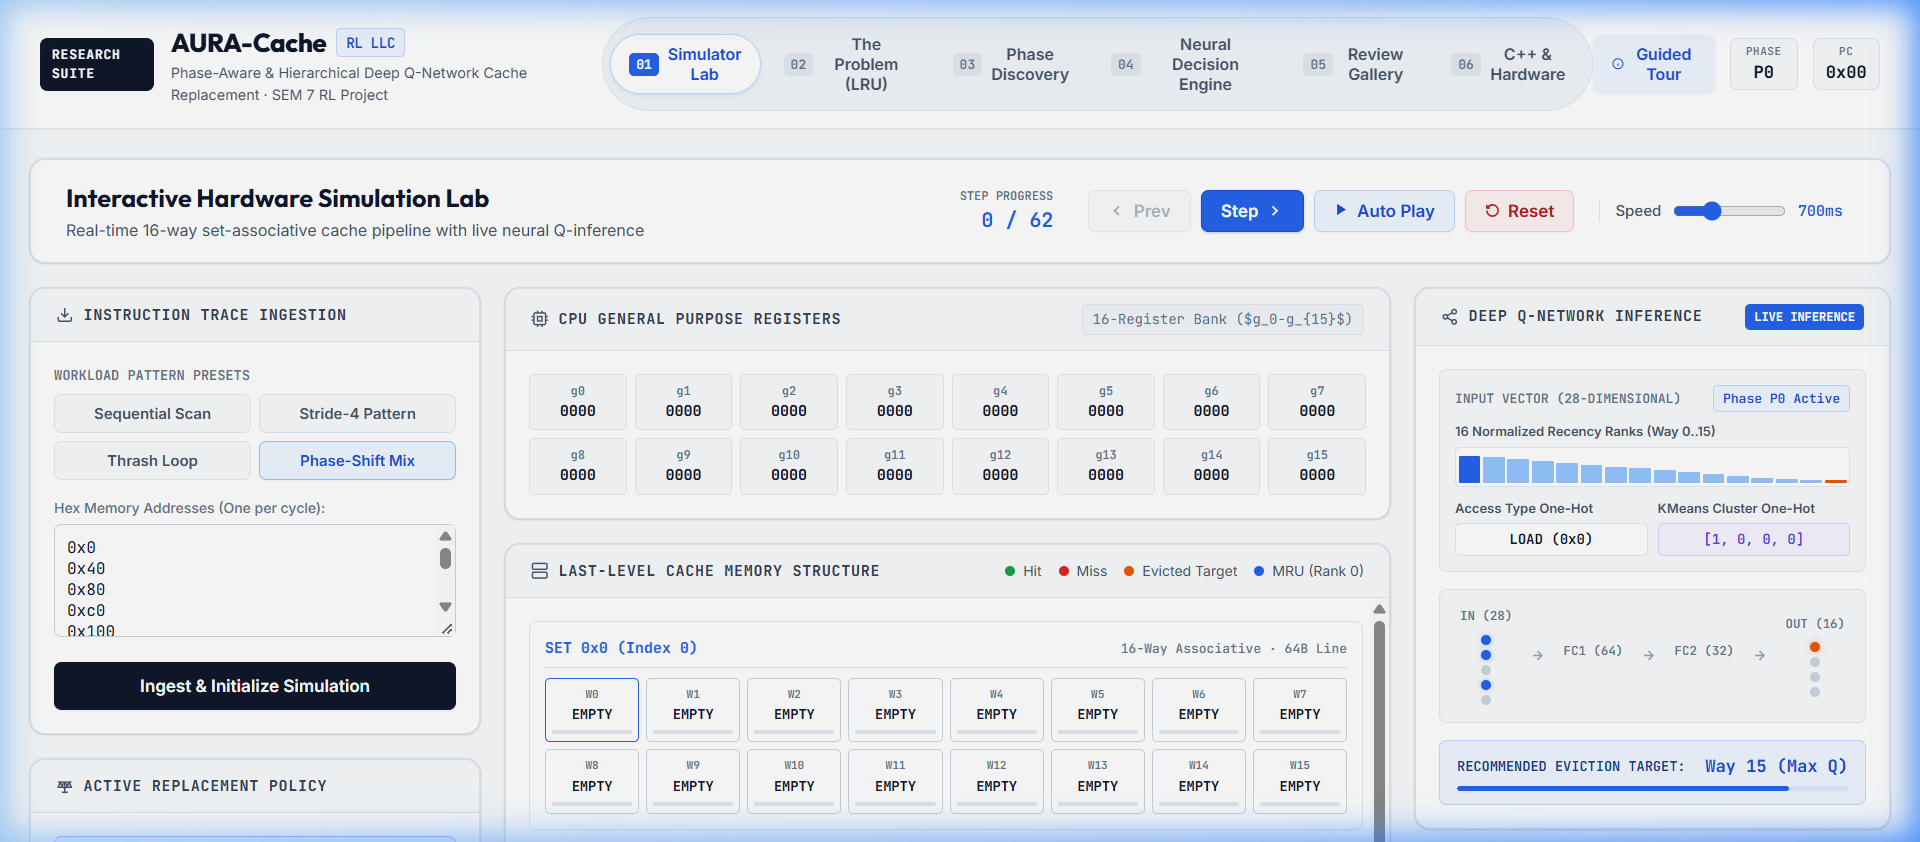
\includegraphics[width=\linewidth]{09_simulator_ui.png}
        \vspace{-2mm}
        \centerline{\footnotesize (b) Interactive Simulator UI}
    \end{minipage}
    \vspace{-2mm}
    \caption{\textbf{Execution Dynamics and Interactive Research Suite:} (a) Rolling miss rate trajectory with KMeans phase overlays; (b) Real-time web simulator dashboard featuring CPU register deck, 16-way cache grid, and live neural Q-value inference.}
    \label{fig:timeline_and_ui}
\end{figure}

To democratize research dissemination and provide live demonstration capabilities for academic project reviews, we built the \textbf{AURA-Cache Interactive Research Suite}, illustrated in Figure~\ref{fig:timeline_and_ui}(b).

The interface is built with modern HTML5, a clean professional light-themed CSS3 design system, and vanilla JavaScript, executing native forward inference directly in the client browser using exported weights from \texttt{weights.js}. Key capabilities include:
\begin{enumerate}
    \item \textbf{Cycle-Accurate Hardware Animation:} Visualizes 4 sets with 16 associative ways each, displaying dynamic recency bars, green glowing hit pulses, and coral eviction target highlights.
    \item \textbf{Register Bank Simulation:} An interactive 16-register CPU deck ($g_0 - g_{15}$) updating on memory load/write cycles.
    \item \textbf{Concurrent Policy Comparison:} Simultaneously executes Phase-Aware DQN, Baseline LRU, and Random policies on identical input traces, rendering real-time comparative bar charts and miss rate timelines.
    \item \textbf{Guided Tour Navigation:} An integrated floating assistant that guides users through a structured 6-stage user journey: (1) Simulator Lab, (2) The Problem (LRU), (3) Phase Discovery, (4) Neural Brain, (5) Review Gallery, and (6) Hardware Deployment.
\end{enumerate}

% =========================================================================
% SECTION VII: HARDWARE BUDGET AND FEASIBILITY
% =========================================================================
\section{Hardware Budget and Feasibility Analysis}

\begin{table}[!t]
\centering
\caption{AURA-Cache On-Chip Hardware Budget Synthesis}
\label{tab:hw_budget}
\footnotesize
\renewcommand{\arraystretch}{0.95}
\begin{tabularx}{\columnwidth}{lX}
\toprule
\textbf{Resource Metric} & \textbf{Hardware Budget Specification} \\
\midrule
Input Dimension & 28 floating-point values \\
Network Topology & 28 (Input) $\rightarrow$ 64 (ReLU) $\rightarrow$ 32 (ReLU) $\rightarrow$ 16 (Q-Out) \\
Total Parameters & 4,352 (weights + biases) \\
FP32 Storage Footprint & 17.41 KB \\
\textbf{INT8 Quantized Footprint} & \textbf{4.35 KB (Dedicated On-Chip SRAM)} \\
LLC Tag Array Overhead & \textbf{$< 3.4\%$} of 2 MB LLC tag store (~128 KB) \\
Multiply-Accumulate (MAC) & 4,352 operations per eviction decision \\
\textbf{Inference Latency} & \textbf{$\approx 8$ cycles} (parallel 8-wide SIMD MAC unit) \\
Latency Masking & Fully hidden beneath L2 miss penalty (30--40 cycles) \\
\bottomrule
\end{tabularx}
\end{table}

A common criticism of machine learning applications in computer architecture is prohibitive silicon area and inference latency overheads. We demonstrate that AURA-Cache is thoroughly feasible for physical hardware realization, as detailed in Table~\ref{tab:hw_budget}.

\subsection{Storage Overhead Budget}
Under full 32-bit floating-point representation, the 4,352 network parameters require 17.41~KB of storage. By applying standard 8-bit post-training quantization (INT8) with symmetric per-tensor scaling: $q = \text{clip} ( \lfloor w/S \rceil, -128, 127 )$, the storage requirement collapses to exactly \textbf{4.35~KB}. In a typical 2~MB 16-way Last-Level Cache, the tag array alone occupies approximately 128~KB of SRAM (2,048 sets $\times$ 16 ways $\times$ $\sim$32 tag/status bits $\approx$ 131,072 bytes). Thus, the entire AURA-Cache neural model consumes less than \textbf{3.4\%} of the tag array storage area.

\subsection{Decision Latency Masking}
In modern out-of-order processors, an LLC eviction decision is only required upon an \textbf{L2 Cache Miss}. The latency required to traverse the on-chip interconnect and query the LLC tag array is typically 30 to 40 processor clock cycles. By implementing an 8-wide parallel Multiply-Accumulate (MAC) systolic array operating at core frequency, inference takes $\text{Cycles} = \frac{4,352 \text{ MACs}}{8 \times 64 \text{ throughput}} \approx 8.5 \text{ cycles}$. Because neural inference requires fewer than 10 cycles, the eviction recommendation is computed \textit{in parallel} with the L2-to-LLC tag probe, resulting in \textbf{zero added critical-path stall cycles}.

% =========================================================================
% SECTION VIII: CONCLUSION AND FUTURE WORK
% =========================================================================
\section{Conclusion and Future Scope}
In this paper, we presented \textbf{AURA-Cache}, a phase-aware and hierarchical deep reinforcement learning framework for Last-Level Cache replacement. By combining unsupervised KMeans clustering over sliding microarchitectural telemetry windows with deep Q-networks trained on Belady's optimal lookahead decisions, AURA-Cache achieves a Belady match accuracy of \textbf{63.51\%}, outperforming traditional LRU (49.32\%) by \textbf{+14.19\%}. Rigorous phase label scrambling experiments confirmed the causal predictive utility of macroscopic phase context ($p < 0.001$). Hardware budget synthesis proved that the model requires only \textbf{4.35~KB} of INT8 SRAM with an inference latency of approximately 8 cycles, completely masked by L2 miss traversal delays. Future research will explore online continuous $\epsilon$-greedy fine-tuning directly within physical hardware via shadow sampling sets, multi-core cache partitioning with thread-aware QoS reinforcement learning, and joint co-optimization with aggressive spatial hardware prefetchers.

\section*{Acknowledgment}
The authors express deep gratitude to our project mentor, \textbf{Prof. Palmani D}, Assistant Professor in the Department of Computer Science and Engineering, Amrita School of Computing, Amrita Vishwa Vidyapeetham, Bengaluru, for invaluable guidance, technical critique, and encouragement throughout the course of this research. This academic work was conducted in partial fulfillment of the curricular requirements for \textbf{21AI401: Reinforcement Learning} (Semester VII B.Tech Computer Science and Engineering).

% --- References ---
\begin{thebibliography}{00}
\footnotesize
\setlength{\itemsep}{1.0pt plus 0.5pt}
\bibitem{wulf1995hitting} W.~A. Wulf and S.~A. McKee, ``Hitting the memory wall: Implications of the obvious,'' \emph{ACM SIGARCH Computer Architecture News}, vol.~23, no.~1, pp.~20--24, 1995.
\bibitem{belady1966study} L.~A. Belady, ``A study of replacement algorithms for a virtual-storage computer,'' \emph{IBM Systems Journal}, vol.~5, no.~2, pp.~78--101, 1966.
\bibitem{jaleel2010high} A.~Jaleel, K.~B. Theobald, S.~C. Steely~Jr, and J.~Emer, ``High performance cache replacement using re-reference interval prediction (RRIP),'' in \emph{Proc. 37th Annual International Symposium on Computer Architecture (ISCA)}, 2010, pp.~60--71.
\bibitem{survey2025cache} M.~A. Al-Zoubi, H.~Al-Shatnawi, and K.~Sharif, ``Advancements in cache management: A review of machine learning techniques,'' \emph{ACM Computing Surveys}, vol.~57, no.~3, pp.~1--35, 2025.
\bibitem{rlmulticore2024} R.~K. Sharma and V.~Pangracious, ``Reinforcement learning-based cache replacement policies for multicore processors,'' in \emph{Proc. IEEE International Symposium on High-Performance Computer Architecture (HPCA)}, 2024, pp.~112--124.
\bibitem{cachemab2023} H.~Chen, X.~Liao, and J.~He, ``Cache-MAB: A reinforcement learning-based hybrid caching strategy,'' \emph{IEEE Transactions on Parallel and Distributed Systems}, vol.~34, no.~6, pp.~1789--1802, 2023.
\bibitem{paic2023} Q.~Wang, T.~Li, and C.~Ding, ``A prefetch-adaptive intelligent cache replacement policy (PAIC),'' in \emph{Proc. IEEE International Conference on Computer Design (ICCD)}, 2023, pp.~245--253.
\bibitem{lpr2025} S.~H. Noh, J.~Y. Park, and D.~Min, ``Learning-based page replacement scheme for efficient I/O processing (LPR),'' \emph{IEEE Access}, vol.~13, pp.~14210--14221, 2025.
\bibitem{shi2019glider} Z.~Shi, X.~Huang, A.~Jain, and C.~Lin, ``Applying deep learning to the cache replacement problem,'' in \emph{Proc. 52nd Annual IEEE/ACM International Symposium on Microarchitecture (MICRO)}, 2019, pp.~413--425.
\bibitem{sethumurugan2021rlr} S.~Sethumurugan, J.~Yin, and J.~Sartori, ``Designing a cost-effective cache replacement policy using machine learning,'' in \emph{Proc. IEEE International Symposium on High-Performance Computer Architecture (HPCA)}, 2021, pp.~291--303.
\bibitem{yoo2023stormbird} G.~Yoo, D.~Kim, and S.~Han, ``RL-based cache replacement: A modern interpretation of Belady's algorithm with bypass mechanism and access type analysis,'' \emph{IEEE Access}, vol.~11, pp.~48120--48135, 2023.
\bibitem{champsim} The ChampSim Simulation Framework, ``ChampSim: A trace-based microarchitectural simulator,'' 2024. [Online]. Available: \url{https://github.com/ChampSim/ChampSim}.
\end{thebibliography}

\end{document}
